%% Copernicus Publications Manuscript Preparation Template for LaTeX Submissions
%% ---------------------------------
%% This template should be used for copernicus.cls
%% The class file and some style files are bundled in the Copernicus Latex Package, which can be downloaded from the different journal webpages.
%% For further assistance please contact Copernicus Publications at: production@copernicus.org
%% https://publications.copernicus.org/for_authors/manuscript_preparation.html


%% Please use the following documentclass and journal abbreviations for preprints and final revised papers.

%% 2-column papers and preprints
\documentclass[journal abbreviation, manuscript]{copernicus}



%% Journal abbreviations (please use the same for preprints and final revised papers)


% Advances in Geosciences (adgeo)
% Advances in Radio Science (ars)
% Advances in Science and Research (asr)
% Advances in Statistical Climatology, Meteorology and Oceanography (ascmo)
% Aerosol Research (ar)
% Annales Geophysicae (angeo)
% Archives Animal Breeding (aab)
% Atmospheric Chemistry and Physics (acp)
% Atmospheric Measurement Techniques (amt)
% Biogeosciences (bg)
% Climate of the Past (cp)
% DEUQUA Special Publications (deuquasp)
% Earth Surface Dynamics (esurf)
% Earth System Dynamics (esd)
% Earth System Science Data (essd)
% E&G Quaternary Science Journal (egqsj)
% EGUsphere (egusphere) | This is only for EGUsphere preprints submitted without relation to an EGU journal.
% Earth Observation (eo)
% European Journal of Mineralogy (ejm)
% Geochronology (gchron)
% Geographica Helvetica (gh)
% Geoscience Communication (gc)
% Geoscientific Instrumentation, Methods and Data Systems (gi)
% Geoscientific Model Development (gmd)
% History of Geo- and Space Sciences (hgss)
% Hydrology and Earth System Sciences (hess)
% Journal of Bone and Joint Infection (jbji)
% Journal of Environmentally Compatible Air Transport System (jecats)
% Journal of Micropalaeontology (jm)
% Journal of Sensors and Sensor Systems (jsss)
% Magnetic Resonance (mr)
% Mechanical Sciences (ms)
% Natural Hazards and Earth System Sciences (nhess)
% Nonlinear Processes in Geophysics (npg)
% Ocean Science (os)
% Polarforschung - Journal of the German Society for Polar Research (polf)
% Proceedings of the International Association of Hydrological Sciences (piahs)
% Proceedings of the International Ocean Drilling Programme (piodp)
% Safety of Nuclear Waste Disposal (sand)
% Scientific Drilling (sd)
% SOIL (soil)
% Solid Earth (se)
% State of the Planet (sp)
% The Cryosphere (tc)
% Weather and Climate Dynamics (wcd)
% Web Ecology (we)
% Wind Energy Science (wes)


%% \usepackage commands included in the copernicus.cls:
%\usepackage[german, english]{babel}
%\usepackage{tabularx}
%\usepackage{cancel}
%\usepackage{multirow}
%\usepackage{supertabular}
%\usepackage{algorithmic}
%\usepackage{algorithm}
%\usepackage{amsthm}
%\usepackage{float}
%\usepackage{subfig}
%\usepackage{rotating}

% Horrible to format J-values.
% Simple species.
\newcommand{\JNO}{\ensuremath{J_{\mathrm{NO}}}}
\newcommand{\JNOO}{\ensuremath{J_{\mathrm{NO_2}}}}
\newcommand{\JNOOO}{\ensuremath{J_{\mathrm{NO_3}}}}
\newcommand{\JNOx}{\ensuremath{J_{\mathrm{NO_x}}}}
\newcommand{\JNNO}{\ensuremath{J_{\mathrm{N_2O}}}}
\newcommand{\JOO}{\ensuremath{J_{\mathrm{O_2}}}}
\newcommand{\JOOO}{\ensuremath{J_{\mathrm{O_3}}}}

% HCHO.
% Full radical rxn.
\newcommand{\JHCHOrFull}{\ensuremath{J_{\mathrm{HCHO} \,+\, h\nu \,+\, \mathrm{2O_2} \,\to\, \mathrm{2HO_2} \,+\, \mathrm{CO}}}}
% Simplified radical rxn.
\newcommand{\JHCHOr}{\ensuremath{J_{\mathrm{HCHO} \,\to\, \mathrm{HO_2}}}}
% Full molecular rxn.
\newcommand{\JHCHOmFull}{\ensuremath{J_{\mathrm{HCHO} \,+\, h\nu \,\to\, \mathrm{H_2} \,+\, \mathrm{CO}}}}
% Simplified molecular rxn.
\newcommand{\JHCHOm}{\ensuremath{J_{\mathrm{HCHO} \,\to\, \mathrm{H_2}}}}

% Other species.
\newcommand{\JCHOCHO}{\ensuremath{J_{\mathrm{CHOCHO}}}}
\newcommand{\JClClOO}{\ensuremath{J_{\mathrm{Cl_2O_2}}}}
\newcommand{\JOCS}{\ensuremath{J_{\mathrm{OCS}}}}
\newcommand{\JSOOO}{\ensuremath{J_{\mathrm{SO_3}}}}
\newcommand{\JISON}{\ensuremath{J_{\mathrm{ISON}}}}
\newcommand{\JmeOO}{\ensuremath{J_{\mathrm{CH_3OO}}}}
\newcommand{\JmeOOH}{\ensuremath{J_{\mathrm{CH_3OOH}}}}
\newcommand{\JmeONOO}{\ensuremath{J_{\mathrm{CH_3ONO_2}}}}
\newcommand{\JmeCHO}{\ensuremath{J_{\mathrm{CH_3CHO}}}}
\newcommand{\JmeCHOmeOO}{\ensuremath{J_{\mathrm{CH_3CHO} \,\to\, \mathrm{CH_3OO}}}}
\newcommand{\JmeCHOCHHHH}{\ensuremath{J_{\mathrm{CH_3CHO} \,\to\, \mathrm{CH_4}}}}
\newcommand{\JmeCOCHO}{\ensuremath{J_{\mathrm{CH_3COCHO}}}}
\newcommand{\JCHHHH}{\ensuremath{J_{\mathrm{CH_4}}}}
\newcommand{\Jpropanal}{\ensuremath{J_{\mathrm{propanal}}}}
\newcommand{\Jacetone}{\ensuremath{J_{\mathrm{acetone}}}}
\newcommand{\JHOBr}{\ensuremath{J_{\mathrm{HOBr}}}}
\newcommand{\JHOCl}{\ensuremath{J_{\mathrm{HOCl}}}}
\newcommand{\JHNOOO}{\ensuremath{J_{\mathrm{HNO_3}}}}
\newcommand{\JHNOOOO}{\ensuremath{J_{\mathrm{HNO_4}}}}
\newcommand{\JHHO}{\ensuremath{J_{\mathrm{H_2O}}}}
\newcommand{\JHHOO}{\ensuremath{J_{\mathrm{H_2O_2}}}}
\newcommand{\JHHSOOOO}{\ensuremath{J_{\mathrm{H_2SO_4}}}}
\newcommand{\JMACR}{\ensuremath{J_{\mathrm{methacrolein}}}}
\newcommand{\JNALD}{\ensuremath{J_{\mathrm{nitrooxy\ acetaldehyde}}}}

% Electronic states of oxygen.
\newcommand{\OP}{\ensuremath{{O(^3P)}}}
\newcommand{\OD}{\ensuremath{{O(^1D)}}}
\newcommand{\JOOP}{\ensuremath{J_{\mathrm{O_2} \,\to\, \OP}}} % O2 -> O(3P)


\begin{document}

\title{Emulation of the United Kingdom Chemistry and Aerosols (version 13.9) Photolysis Schemes (FASTJ-X vn2.X?) with a Random Forest}


% \Author[affil]{given_name}{surname}

\Author[1][st838@cam.ac.uk]{Sophie}{Turner} %% correspondence author
\Author[1, 2]{Luke}{Abraham}
\Author[1, 2][ata27@cam.ac.uk]{Alexander T.}{Archibald}

\affil[1]{Centre for Atmospheric Science, Yusuf Hamied Department of Chemistry, University of Cambridge, Cambridge, UK}
\affil[2]{National Centre for Atmospheric Science, Leeds, UK}


%% The [] brackets identify the author with the corresponding affiliation. 1, 2, 3, etc. should be inserted.

%% If an author is deceased, please add \deceased[$Deceased date if applicable$]{$Author number$} (e.g. \deceased[13 November 2015]{2}) at the end of the affiliations. The author number depends on the placement of the author in the author list, e.g. the third author has number 3.


%% If authors contributed equally, please add \equalcontrib{$Author numbers$} (e.g. \equalcontrib{1,3}) at the end of the affiliations. The author number depends on the placement of the author in the author list, e.g. the third author has number 3.




\runningtitle{Random Forest Emulation of UKCA Photolysis}

\runningauthor{Turner et al.}





\received{}
\pubdiscuss{} %% only important for two-stage journals
\revised{}
\accepted{}
\published{}

%% These dates will be inserted by Copernicus Publications during the typesetting process.


\firstpage{1}

\maketitle



\begin{abstract}

% Atmospheric photolysis.
Atmospheric photolysis directly affects air pollution and significantly influences the mechanisms of climate change.

% What's UKCA and UM.
The Unified Model (UM) is the atmospheric science component of the United Kingdom's Earth System Model (UKESM), an internationally important coupled climate model. The United Kingdom Chemistry and Aerosols (UKCA) project is the chemistry component of the UM and performs the simulation of photolysis.

% Problem.
Among the various components of UKCA, photolysis is known to be computationally demanding. It involves numerous calculations that encompass different chemicals, locations, altitudes, and time steps, making up approximately 20\% of UKCA's run-time, and approximately 25\% of UKCA's time spent on scientific calculations. Enhancing the efficiency of photolysis simulations could lead to faster execution of the entire Earth system model and reduce power consumption. 

% Aims.
The primary objective of this project was to develop a machine learning model to accelerate UKCA photolysis without compromising its accuracy.

% What was done.
UKCA photolysis rate coefficients for multiple reactions were emulated using a random forest which was trained offline in python using physical input data from the UM, including shortwave solar fluxes, solar zenith angle and other relevant data. A proof of concept version of the random forest was then integrated into UKCA in Fortran and run online in the UM. 

% Accuracy.
The random forest was able to emulate UKCA photolysis rate coefficients accurately, with a coefficient of determination of 0.97 compared to the original scheme over all emulated reactions, and 0.76 to over 0.99 for individual reactions. 

% Speedup.
The random forest photolysis scheme ran seven times faster in UKCA than the main existing photolysis scheme, Fast-JX, and the whole UM ran 1.97\% faster, potentially allowing an extra four weeks of simulation per real day.

\end{abstract}


%\copyrightstatement{TEXT} %% This section is optional and can be used for copyright transfers.


\introduction %% \introduction[modified heading if necessary] 

\subsection{Photolysis in UKCA}

% Atmospheric photolysis.
Atmospheric photolysis refers to the phenomenon in which molecules in the atmosphere are dissociated by solar radiation. As a result of some common photolysis processes, radicals are formed, which are very reactive species, and they rapidly initiate subsequent atmospheric reactions \cite{finlayson-pitts_chemistry_2000}. This has considerable implications for air pollution. Atmospheric photolysis reactions affect phenomena such as smog in urban areas, and the thinning of the stratospheric ozone layer, which seriously impact the health of people and the environment \cite{seinfeld_atmospheric_2016}. Including photolysis in climate models is necessary for obtaining accurate predictions of changes in atmospheric composition. The rates of photolysis reactions are influenced by various factors, including clouds, aerosols, atmospheric pressure and the time of day and year \cite{liang_chemical_2013}. All of these factors must be carefully taken into account when developing a comprehensive model that simulates this process.

% How photolysis is calculated.
The calculation of photolysis rates involves determining the intensity of solar radiation at different wavelengths, quantifying the absorption cross-sections of the molecules and accounting for factors such as atmospheric composition, altitude, latitude, time of day and season. It is beneficial to isolate and focus on the rate coefficient of this process to avoid confusion caused by other factors, such as changes in concentration of the chemicals over time. The rate coefficient of the photolysis reaction is termed `J' and has units of $s^{-1}$. The rate coefficient is also referred to as the J-value, J rate, rate constant, or frequency. The term, `J-value', is used in this work. The J-value of a particular photolabile chemical, which absorbs light in a specific range of wavelengths, can be calculated as
\begin{equation}
J = \int_{0}^{\infty} \Phi (\lambda, T) \sigma (\lambda, T) F (\theta, \lambda) d \lambda 
\end{equation}
\addcontentsline{equ}{myequations}
{\protect\numberline{\theequation}Photolysis rate coefficient}
where $\Phi$ is the quantum yield for photolysis of the chemical, $\lambda$ is the wavelength, $T$ is the temperature, $\sigma$ is the absorption cross-section, $F$ is the flux of light, also known as the actinic flux, $\theta$ is the solar zenith angle and $d \lambda$ is the change in wavelength \cite{king_calculating_2013}. Flux refers to the difference in the amount of radiation reaching the molecule over time, which varies significantly at a point over the course of a day.
At a point in space and time in the atmosphere, the solar zenith angle (SZA) is the angle between the direction of incoming solar radiation and the local vertical line perpendicular to the Earth's surface at that point \cite{finlayson-pitts_chemistry_2000}. 
J-values can range from around $10^{-16} s^{-1}$ to over $10^{-2} s^{-1}$ and vary greatly with altitude.

% UKESM, UM and UKCA.
The United Kindgom Earth System Model (UKESM) is a collaborative initiative involving the Met Office, the National Centre for Atmospheric Science (NCAS) and the UK academic community \cite{sellar_ukesm1_2019}. UKESM plays an important role in assessing climate forcing, conducting projections on air quality and quantifying the impacts of mitigation measures. It contributes to the Coupled Model Intercomparison Project \cite{eyring_overview_2016}. The atmospheric component of UKESM is the Unified Model (UM), developed by the Met Office, while the United Kingdom Chemistry and Aerosols (UKCA) model \cite{archibald_description_2020} serves as its atmospheric chemistry and aerosol component. The UM and UKCA code is extensive and complicated due to a variety of chemistry schemes and photolysis approaches, and there are various UM versions and many configurations that run on different computing infrastructures.

% Photolysis schemes in UKCA and how they work.
Different schemes are present in UKCA for photolysis calculations, including a legacy `2D' scheme based on the interpolation of tabulated values pre-calculated in the Cambridge 2D model \cite{abraham_united_2014}, and the Fast-JX scheme \cite{telford_implementation_2013}, suitable for tropospheric and stratospheric conditions. The primary photolysis scheme currently used in UKCA is Fast-JX, which is a more advanced and precise approach. % Strat scheme.
Fast-JX is intended to be used at atmospheric pressures greater than 20 Pa \cite{wild_fast-j_2000} and most photolysis occurs within this region. When using Fast-JX in the UM for configurations which include altitudes at which atmospheric pressure drops below 20 Pa, there are three options for how to handle the portion of lower pressure; Fast-JX may be used, photolysis may be approximated using the lookup table of stratospheric rates, or both Fast-JX and the lookup table may be used and their results aggregated.
The most accurate of the options at pressures less than 20 Pa is considered to be the combination of both Fast-JX and the lookup table scheme. Hence, the emulation should, ideally, not only emulate Fast-JX, but also emulate the combined results of Fast-JX and the lookup table in the upper stratosphere.

\begin{figure}
    \centering 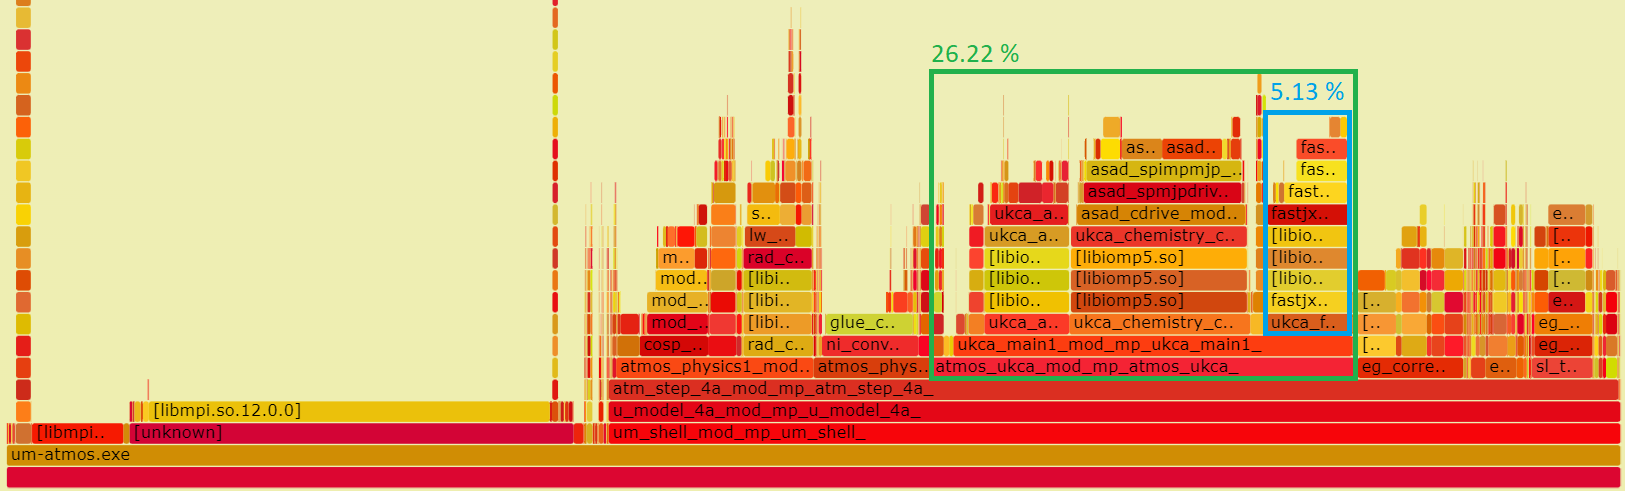
\includegraphics[width=\textwidth]{images/flame.png}
    \caption{\textit{Flame graph showing the timed processes during a run of the UM, from Dichev and Tamerus (2021) \cite{dichev_report_2021}. UKCA and photolysis are highlighted in green and blue, respectively, with their total percentages of the UM's run-time.}}
    \label{flamegraph}
\end{figure}

% Timings.
Among the various components of UKCA, photolysis is known to be computationally demanding. It involves numerous calculations that encompass different chemicals, locations, altitudes and time steps, making up approximately 20\% of UKCA's run-time, and about 25\% of UKCA's time spent on scientific calculations \cite{dichev_report_2021}. In each grid box, there is incoming and outgoing light, which can occur either directly or through scattering, involving neighbouring grid boxes. These effects can propagate across multiple boxes of the grid. The photolysis calculating routines are invoked for each grid box at hourly UKCA time steps. The flame graph in Figure \ref{flamegraph} shows an example of the timed processes during a run of the UM, of which photolysis accounts for 5.13\% of the total run-time \cite{dichev_report_2021}. These vary depending on the chemistry scheme chosen, the type of suite run and other options selected for the run. For this benchmark, an atmosphere-only configuration of the UM was used, with the StratTrop chemistry scheme \cite{archibald_description_2020}, on the Cambridge Service for Data Driven Discovery 3 (CSD3) HPC with 56 central processing unit (CPU) cores and with no specifically dedicated parallelism \cite{cambridge_service_for_data_driven_discovery_research_2025}.  

% Power usage, electricity bill cost and GWP.
Reducing energy usage is a priority for climate modellers and high-performance computing (HPC) centres. Running models such as UKESM in typical scientific workloads, comprising many multi-decadal simulations, requires megawatts of energy, incurring a global warming potential of tonnes of CO$_2$ equivalent greenhouse gas emissions (CO$_2$e) and financial costs of tens of thousands of GBP which often belong to the taxpayers \cite{jackson_emissions_2023}. Improving the computational efficiency of processes within the model, including photolysis, is essential for reducing its energy consumption.

% Why speed it up.
If significant progress is made to speed up photolysis simulations, it could open up new possibilities for studying the complex chemistry-climate dynamics within the coupled Earth System over extended periods, spanning multiple centuries.

\subsection{Random Forests}

% ML getting popular.
Machine learning applications can efficiently process large datasets, emulate complex computations involved in simulations and learn from existing data patterns and relationships to make predictions and optimise calculations. This could potentially reduce the computational burden and time required for photolysis calculations. Additionally, ML could help identify key factors and parameters that influence photolysis, enabling the development of more efficient algorithms and models. The realm of ML is extensive and growing, offering innumerable possibilities and methodologies to pursue. An objective of this project is to narrow down these options and determine the most suitable approach. Many ML methods suffer from the same drawbacks; for example, supervised ML tends to struggle with extrapolation, as it often fails to accurately predict conditions that lie beyond the range of the training data.

% How emulation works.
ML parameterisations, such as emulation, can reduce the need to balance correct physics with time-saving simplifications \cite{lagerquist_using_2021}. Emulation involves a surrogate model that can statistically predict the outcome of the simulation, with faster execution. Machine learning emulators that are trained using model-simulated data and aim to mimic existing parameterisations may not need additional physical constraints. This is because the simulated data already incorporate the necessary physical constraints implicitly. A common problem with emulation of atmospheric models is error accumulation as the period of simulated time increases beyond a few days \cite{krasnopolsky_using_2022}.

% What was done.
Data were preprocessed and feature selection tests were repeated using an algorithm relevant to the random forest. 
The random forest was designed and tuned, and tests were conducted on different spatial dimensions of data, and day and night data. Single and multiple output models were compared and the 2D stratospheric photolysis scheme was emulated as well as Fast-JX. 
Relationships between inputs and outputs and profiles of vertical columns were investigated.
Possibilities to improve the model were assessed, including standardising targets, correcting altitude, scaling SZA and adding ozone column and additional cloud information as input features. Patterns and causes of error and bias were addressed. An in-depth evaluation of model performance was conducted for each experiment.

A random forest was trained to enable integration of a proof of concept version of the emulator into the UM. The ML model's data were imported into the UM and a new module was added to the UKCA code for the emulated photolysis scheme. The emulator was tested in the UM and outputs were compared to outputs with the original photolysis scheme, for J-values and relevant downstream chemistry and physics parameters. Both schemes were also timed within the UM and UKCA, and the machine learning photolysis scheme was faster than the original simulation. Tasks were identified which must be carried out in the future in order to fully integrate a random forest emulator into the UM for operational use.

% Diagram of a decision tree.
\begin{sidewaysfigure}[htpb]
    \centering 
    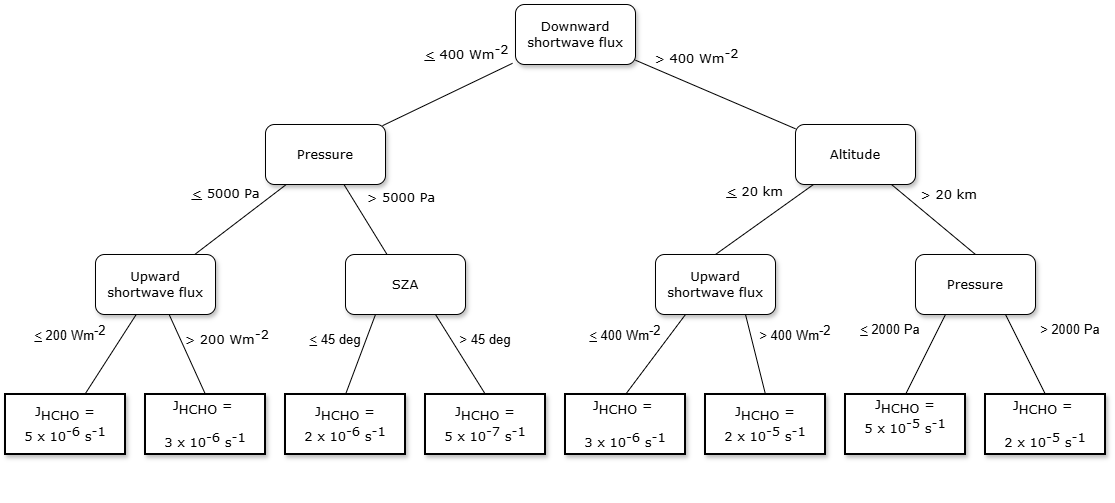
\includegraphics[width=\textheight]{images/Tree.png}
    \caption{\textit{An example of a decision tree predicting $J_{HCHO}$. This tree has 15 nodes, 8 leaf nodes and a depth of 3. The threshold and prediction values displayed are arbitrary dummy values with no scientific basis.}}
    \label{tree diagram}
\end{sidewaysfigure}

% Explain what a decision tree is.
A decision tree is a model containing many nodes, which iteratively compares the value of an input feature for each sample to a threshold value at every node and traverses a path through the tree depending on whether the input feature value exceeds the threshold value at each node, ending at a leaf node which contains a prediction value for the output feature \cite{tibshirani_elements_2001}. Each node considers one randomly chosen input feature. A top-down, greedy binary decision tree was used, in which each parent node has two child nodes, with an input feature value less than or equal to the node's threshold leading to the left child and a value higher than the threshold leading to the right child. Figure \ref{tree diagram} represents a simplified example of this process. The tree shown in the Figure is a single-output model but a decision tree can also output a vector of prediction values at leaf nodes for a set of output features.

% Show maths eqns.
Chosen splits minimise the loss function at each node, $m$. 
% MSE.
With the MSE loss function, the algorithm at each node minimises the equation,
\begin{equation}
 \sum_{i\epsilon R^{left}_{m}}(y_i - \bar{y}_{left})^2 + 
   \sum_{i\epsilon R^{right}_{m}}(y_i - \bar{y}_{right})^2
\end{equation}
\addcontentsline{equ}{myequations}
{\protect\numberline{\theequation}MSE loss function in a decision tree}
where $R^{left}_{m}$ is the left split and $R^{right}_{m}$ is the right split at node $m$, $y$ is the target value and $\bar{y}$ is the mean of the values in the node. This is done for the set of samples which reach the node during the training process.
At each leaf node, the prediction is the mean of the target values of samples reaching that leaf. 
The mean of the squared errors of predictions to targets is used as the performance metric.

% Explain what random forest is.
A random forest was explored as an alternative tree-based method. A random forest is an ensemble of decision trees, in which each tree is trained on a subsample of the data and input features, and the output is the mean of the outputs from every tree \cite{james_introduction_2023}.

% Why might it be useful?
A benefit of using a random forest rather than a single decision tree is the expansion of values which can be output by averaging the leaf node values from every tree. This results in a smoother transition between potential output values, allowing the outputs to appear almost continuous rather than obviously discrete. Furthermore, each tree in a random forest may be more efficient to train, store in memory and traverse than a single decision tree when trained on subsets of features. For example, if each tree is trained on two randomly selected input features out of ten, the depth of tree growth should be far less than that of a single tree trained on all ten input features. Although random forests do not explicitly learn relationships between features, each tree may be able to learn more specific patterns caused by the two selected input features than could a single decision tree.   

\subsection{Aims of Project}

Enhancing the efficiency of photolysis simulations could lead to faster execution of the entire Earth system model and potentially reduce power consumption. This project aims to determine whether ML can adequately emulate an atmospheric photolysis model and identify suitable ML methods to do this. Ultimately, the objective is to use the chosen ML method to accelerate UKCA photolysis without compromising its accuracy. 

Assuming a simulation throughput of approximately four model years per real day, even a 1\% improvement in overall UM performance would be significant, potentially enabling an additional two weeks of simulated time per real day and considerably reducing cumulative energy and financial costs. Accordingly, this project aims for an overall UM speedup of 1\%, corresponding to approximately a 4\% speedup of UKCA and approximately a 20\% speedup of photolysis.

The target predictive skill of the emulator is to achieve a coefficient of determination of at least 0.9 for every reaction, in line with high-performing models in recent literature \cite{liu_deep_2025} \cite{pan_development_2025}, ideally throughout the spatial and temporal range of the test data. This aim is ambitious because the model must emulate photolysis throughout the whole global grid up to a height of 85 km and in all atmospheric conditions, which is a more complex task than those described in the literature. Emulator error is additional to the intrinsic error of the underlying model though, such that total deviation from observations may be larger in practice.
A list of emulated photolysis reactions is provided in Appendix \ref{rxns}.\\

The specific research aims are:\\

1. Identify an appropriate ML model to emulate UKCA photolysis rate coefficients. This is mainly covered in the second chapter.\\

2. Use the chosen method to accurately emulate UKCA photolysis rate coefficients, with a global coefficient of determination of at least 0.9 for each emulated reaction. This is mostly addressed in the third chapter.\\

3. Use the chosen model to speed up the run time of UKCA within the UM, reducing the run time of the photolysis portion of UKCA by at least 20\%. This is covered in the fourth chapter.

\subsection{Performance Metrics}

% R2 
The main accuracy metric chosen for model assessment was the coefficient of determination, also known as the \RR\ score, which measures the proportion of variance in the dependent variable that is predictable from the independent variables \cite{draper_applied_1998}. 
% The maths of what R2 is.
The coefficient of determination is defined as 
\begin{equation}
R^2 = 1 - \frac{RSS}{TSS}
\end{equation}
\addcontentsline{equ}{myequations}
{\protect\numberline{\theequation}Coefficient of determination} 
where $RSS$ is the residual sum of squares, which measures the error, and $TSS$ is the total sum of squares, which is proportional to the variance of the data.
The residual sum of squares is
\begin{equation}
  RSS = \sum_{i=1}^{n}(y_i - \hat{y}_i)^2
\end{equation}
between the true targets, $y$, in the dataset and the values predicted by the model, $\hat{y}$, for the number of data points, $n$. 
The total sum of squares is similar, but for the mean of the true values, $\bar{y}$:
\begin{equation}
  TSS = \sum_{i=1}^{n}(y_i - \bar{y})^2
\end{equation}
An \RR\ score of one is a perfect prediction. An \RR\ score of zero means the model performed no better than if it had predicted the mean, whereas a negative \RR\ score means the model performed worse than if it had predicted the mean. 
It was chosen as the main metric because it is widely used and intuitively understood for regression problems and because it is applicable to all ML models, datasets and targets, unlike many other accuracy metrics, which are specific to the ML method, the dimensions of the data, or the scale of each target, and therefore do not produce comparable results across different experiments and target J-values. 
Using the \RR\ score as an accuracy metric sometimes makes predictions appear poor for the smallest photolysis rates. It is useful to also visualise the data in plots and use additional metrics to gain a better understanding of the accuracy and fit.

\section{Method}

\subsection{Data and Preprocessing}

% Dataset.
A dataset was compiled from UKCA outputs, encompassing significantly more data than the sample used in the linear regression experiments, for training a machine learning model. All J-values calculated by the StratTrop chemistry scheme were output, rather than just those comparable to ATom data which were previously used. Code was also written to output all additional and intermediate J-values from the CRI-Strat2 chemistry scheme in case it was later used. Four days of data were retrieved from a nudged SSP simulation. They were each at a resolution of 24 hours, 85 vertical levels, 144 latitudes and 192 longitudes, and contained 83 fields of J-values and fields related to photolysis. 33 of the J-values output from the UM were only available in CRI-Strat2 and not StratTrop, and output J-values of zero in all data from StratTrop runs. They were not necessary because they were intermediate species and contained the same functional groups as other species output from StratTrop, meaning they used the same base J-values from Fast-JX.

% Flattening.
The Scikit-Learn Python package was used for quick development and testing of different ML methods because it provides a vast library of pre-built models of various ML algorithms, which can easily be adjusted in Python \cite{pedregosa_scikit-learn_2011}. Other packages tend to be specifically designed for one approach, such as neural networks, and lack the range of tools and generalisability available from Scikit-Learn. For most applications, Scikit-Learn requires input data to be structured as a two-dimensional array, in which one dimension is samples and the other is features. The output data from the UM were five-dimensional, with dimensions of time, altitude above sea-level, latitude, longitude and field. `Field' is the name given to output items, such as each J-value and physical parameters from the UM. The data were flattened from five dimensions to two without losing the spatial or temporal information by including all fields, as well as time, altitude, latitude and longitude as features in the resulting array. This flattening required data to be padded, which was specifically done in the same order of dimensions as the UM's output data. This repetition did not increase the size of the data because it is representative of the standard one-dimensional, contiguous storage of the data at a lower level, resulting in the same number of elements. This structure allowed the dimension values themselves (time, altitude, latitude and longitude) to be included as rows in the matrix of potential training data, treated in the same way as the other fields. A risk identified of this approach was that repeating some values over many samples could bias the ML models, depending on the ML techniques chosen. Nevertheless, the dataset was constructed with the intention of suitably sampling from it when training each ML model. The surface-level solar zenith angle was also repeated up each vertical column. The flattened data were saved as numpy arrays in .npy files to enable fast reading, writing and computation in Python \cite{harris_array_2020}. A metadata file was written during this process to explain the data structure. 

% Physical data.
Physical data from the UM were used as model inputs, including temporal and spatial data as well as the pressure, shortwave flux, SZA, temperature, humidity and cloud fraction of each sampled point.

% 1 year.
The emulator was intended to be trained on UM output from at least one simulated year to ensure seasonal patterns were captured. The training dataset must also be sampled at a high enough resolution to capture diurnal patterns, because conditions including the flux of light and cloud cover at a point vary considerably throughout the day.

% Raw data size.
Each file of one-day outputs from the UM contained data from 24 timesteps, 85 model levels, 144 latitudes, 192 longitudes and between 35 and 88 output fields, depending on the completeness of data detail desired for the chosen machine learning method, including input and target features. This resulted in a dataset containing between approximately 56 million and 4.7 billion data points in a file of up to 18 GB of single-precision data for each simulated day. A year of output data occupied up to 6.5 TB of storage. It was then necessary to sample the one-year dataset to reduce its size.

% Conclusion.
Low-resolution data from every day of the year, sampled either randomly or systematically, appeared to form the most comprehensive dataset. Due to the vastness of available data, more advanced sampling techniques were not deemed necessary.

% Day-file sampling.
According to the final design, each day of data in one year was sampled individually, from uniform random indices, to form an appropriately-sized subsample of 500,000 daily data points. The subsamples from each day were then joined to form one file containing a single-precision numpy array of all features and samples from the year's dataset.

% Final design.
Night-time data points with no sunlight present and the upper stratosphere at pressures below 20 Pa were retained in the sampled dataset.

\subsection{Model Design}

Both of the photolysis models in UKCA, Fast-JX and the stratospheric lookup-table, were emulated by the random forest to produce a single photolysis scheme for all altitudes.

Arranging the input data into a two-dimensional matrix of samples and features allowed the random forest to be transferable to different spatial dimensions and timestep frequencies. A grid box, a column, the entire global grid, or any shaped sample of the grid can be passed to the random forest without any added processing required. The UM calls photolysis on MPI domains which are typically a subset of the Earth grid, split by latitude and longitude, with full columns retained. The low-resolution N48 version of the UM which runs on the VM splits its grid into four domains by halving the grid by both latitude and longitude, allowing processing by a personal computer. The higher-performance N96 versions of the UM split the grid into more domains, depending on the configuration and infrastructure used. The random forest's data structure makes it transferable to these domains as well as any other grid shape, such as a single-column model. This is preferable to physics-based photolysis models which require specific spatial dimensions and timestep frequencies.

% Single.
A single random forest could predict all reactions from all inputs, or an individual random forest could predict each reaction or the reactions of each functional group or otherwise similarly-behaving species. The main benefit of a single model which predicts every reaction is computational efficiency; decision trees are traversed based on input feature values and the leaf nodes hold one-dimensional arrays of prediction values, so a random forest of the same structural size takes practically the same amount of time to predict many targets as to predict one target. In reality, the random forest structure required to do this may be larger than would be required to predict one target, so one forest predicting all reactions' J-values would likely be somewhat slower to traverse than one which predicts the J-values of one reaction, but still much faster than a large ensemble of single-output random forests.

% Tuning.
The random forest design was tuned by adjusting number of trees, depth of trees, number of leaves, proportion of training data seen by each tree, number of input features passed to each tree, fitness function and pruning complexity parameter. 

\begin{figure}[htpb]
    \centering 
    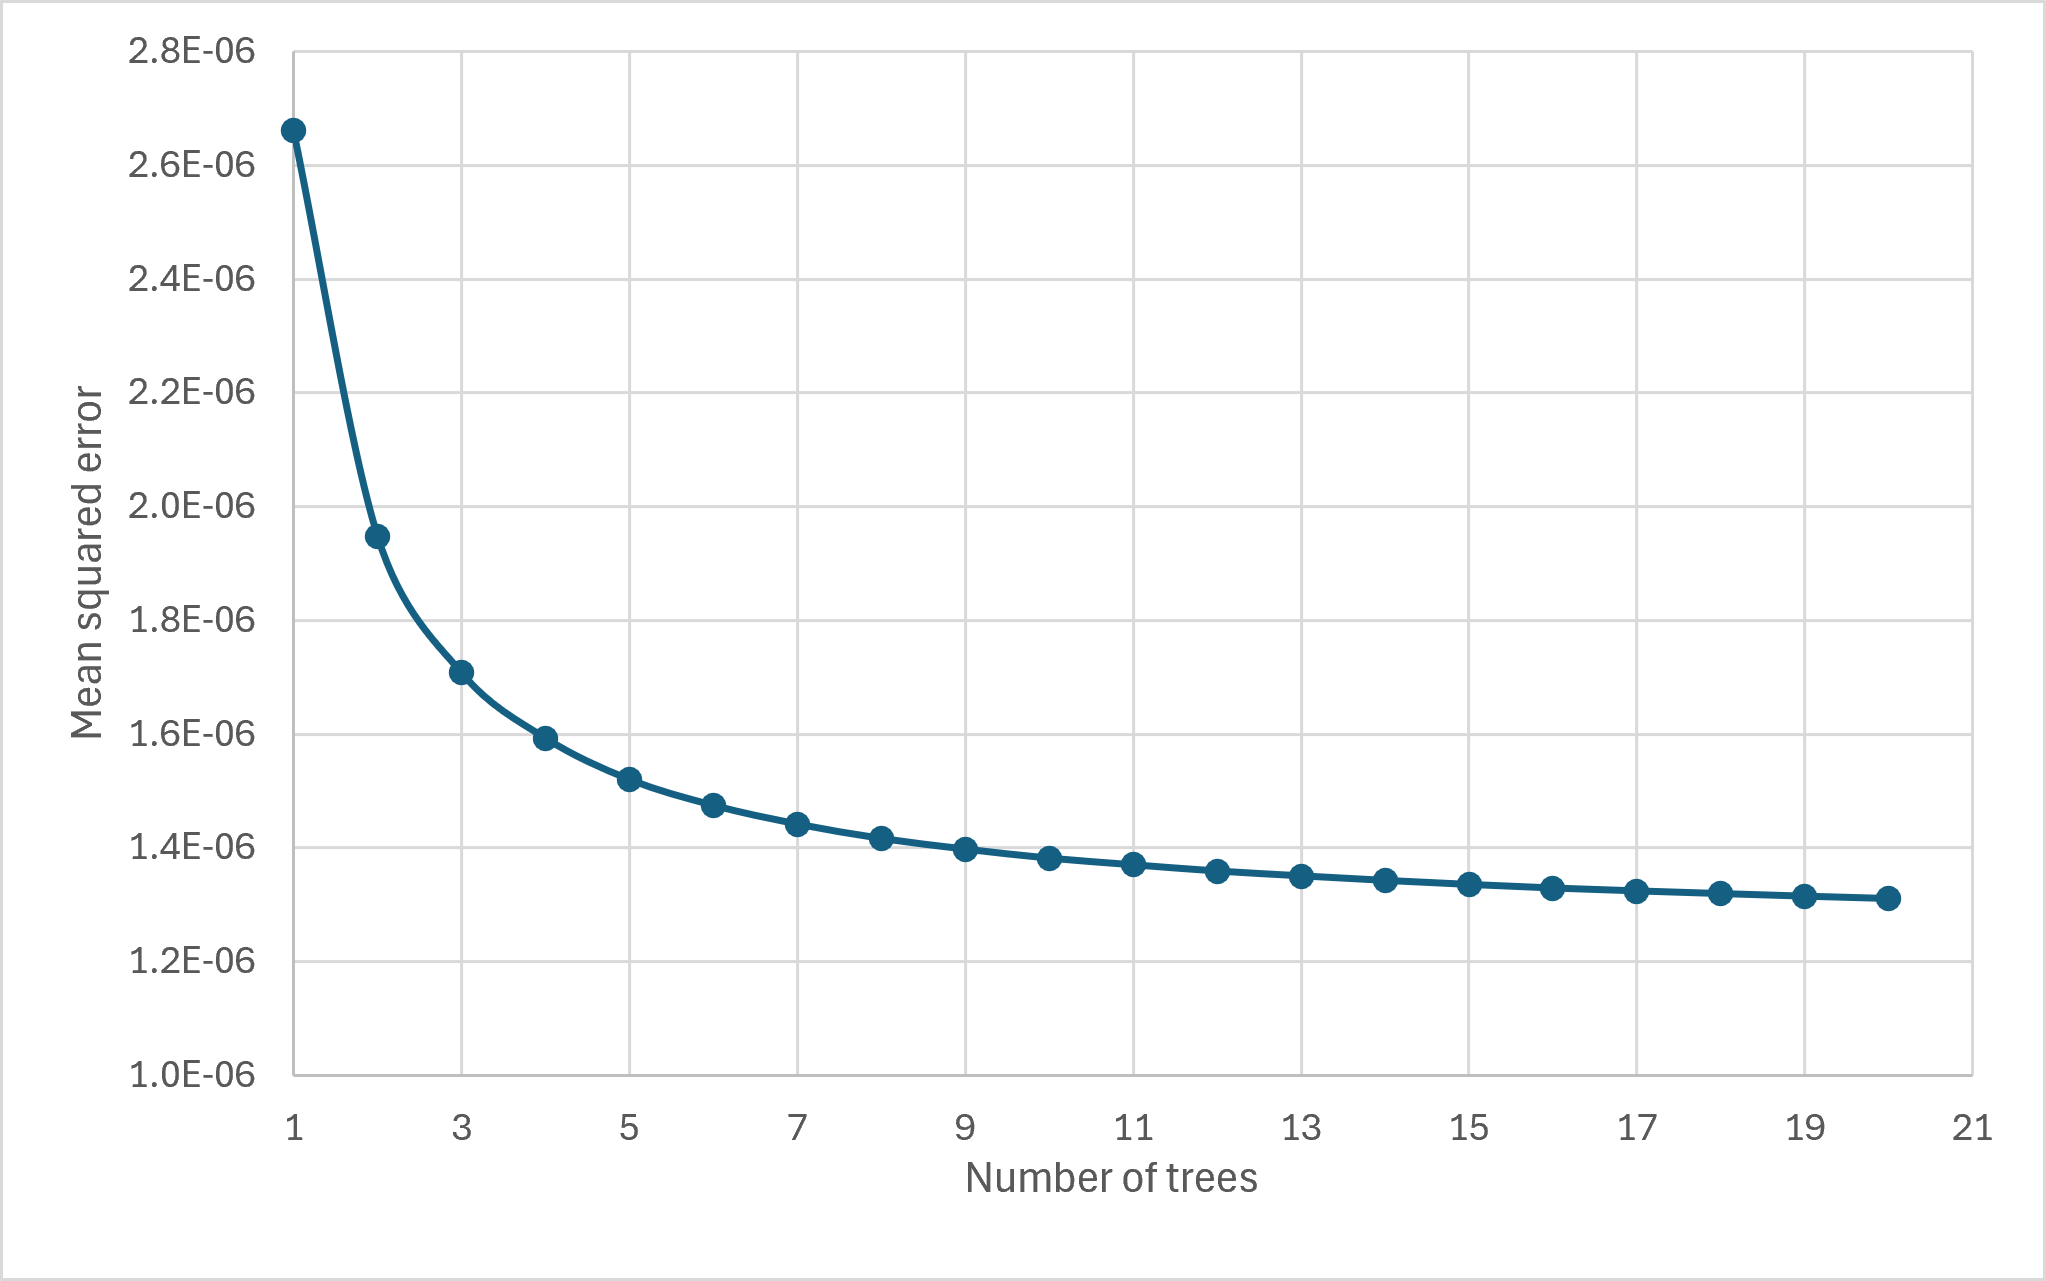
\includegraphics[width=\linewidth]{images/Forest n trees MSE.png}
    \caption{\textit{MSE of random forests of 1 to 20 trees, predicting a representative subset of reactions (\JHCHOr, \JOOO, \JNOO, \JNOOO, \JHOCl\ and \JHHOO) from physical inputs in a global sample of one year of data.}}
    \label{n trees MSE}
\end{figure}

\begin{figure}[htpb]
    \centering 
    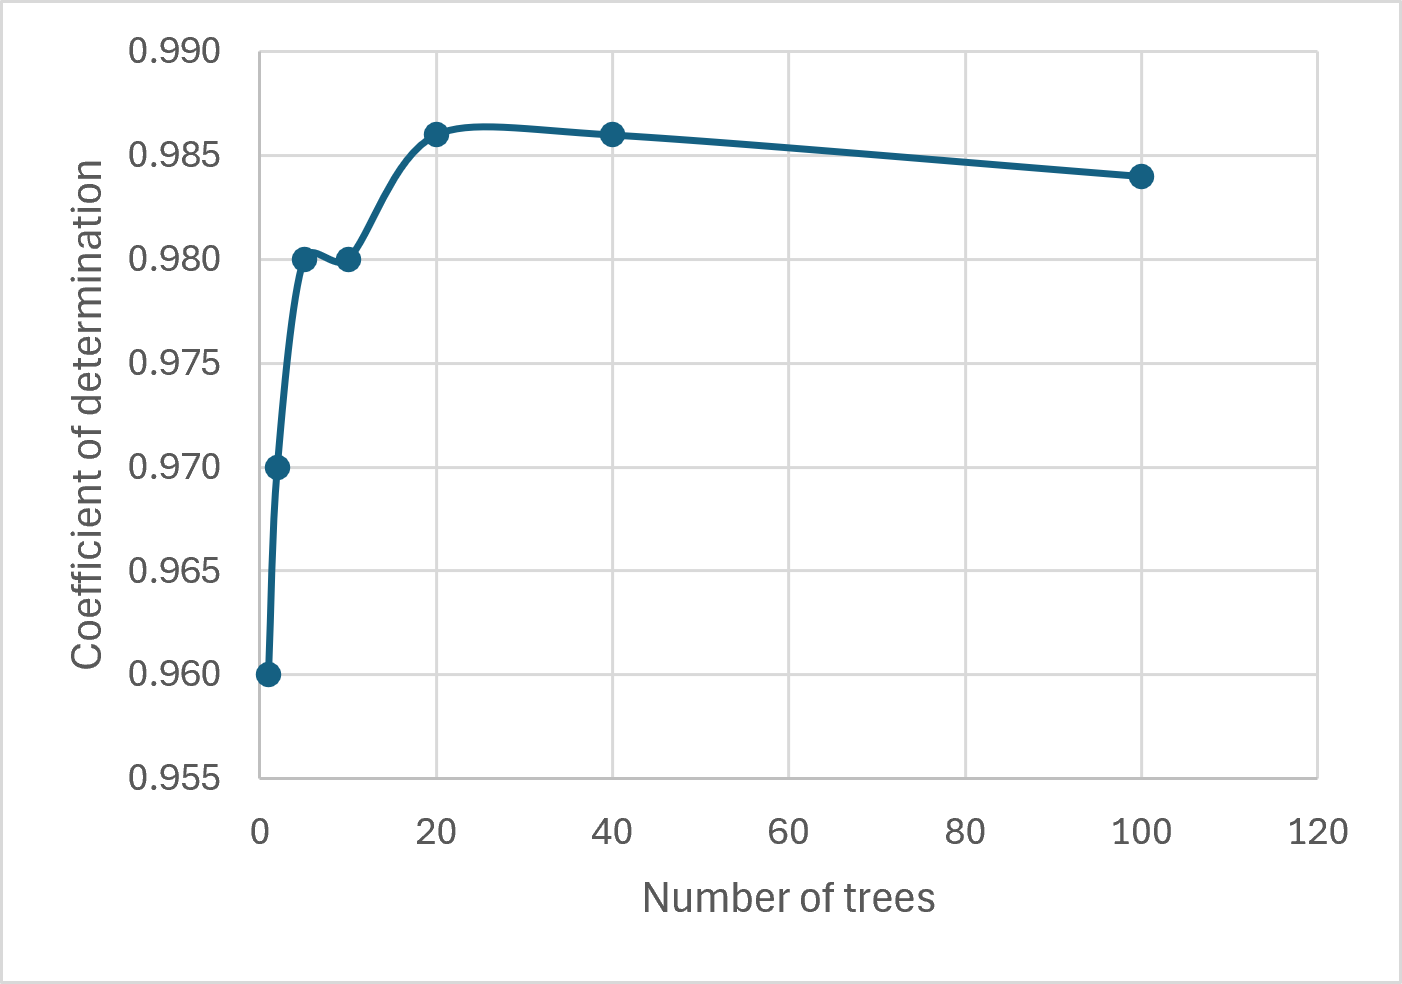
\includegraphics[scale=1.1]{images/n trees R2.png}
    \caption{\textit{Mean \RR\ scores of predictions to targets from random forests containing different numbers of trees, from 1 to 100. Physical inputs were used to predict all J-values in a global sample of one year of data.}}
    \label{n trees R2}
\end{figure}

\begin{table}[htbp]
\centering
\caption{\textit{A summary of random forests' performance using different numbers of trees from 1 to 2000, while keeping the memory usage similar by adjusting the size of the trees in the forest. Physical inputs were used to predict all J-values in a global sample of a year of data. `Max samples' is the proportion of training data samples provided to each tree, randomly sampled from the full training dataset.}}
\resizebox{\textwidth}{!}{
\begin{tabular}{|lccccc|}
\hline
Test description & Trees & Max samples & Max leaf nodes/tree & $R^2$ & MSE / $s^{-2}$ \\
\hline
Baseline & 1 & None (all) & 200000 & 0.960 & $4.17 \times 10^{-7}$ \\
Increase n trees & 20 & 0.2 & 10000 & 0.986 & $3.98 \times 10^{-7}$ \\
Increase n trees & 40 & 0.2 & 5000 & 0.986 & $4.09 \times 10^{-7}$ \\
Increase n trees & 100 & 0.2 & 2000 & 0.984 & $4.22 \times 10^{-7}$ \\
Increase n trees & 1000 & 0.2 & 200 & 0.971 & $4.86 \times 10^{-7}$ \\
Increase n trees & 2000 & 0.2 & 100 & 0.962 & $5.21 \times 10^{-7}$ \\
Best above w/ double tree size & 20 & 0.2 & 20000 & 0.987 & $3.87 \times 10^{-7}$ \\
Best above w/ double n trees & 40 & 0.2 & 10000 & 0.986 & $3.98 \times 10^{-7}$ \\
\hline
\end{tabular}}
\label{n trees table}
\end{table}

% Forest size.
Random forests were constructed and tested with 5 input features and 1 to 50 trees. Figures \ref{n trees MSE} and \ref{n trees R2} exhibit MSE and \RR\ scores of predictions to targets from random forests containing different numbers of decision trees. Table \ref{n trees table} details the effect of increasing the number of trees while reducing the size of each tree in order to maintain similar memory usage. For most J-values, the random forest performed best with 5 to 20 trees, with 20 trees identified as the ideal for a multi-output model predicting all J-values.

% Depth > size.
Tests on the random forest configuration indicated that model performance was more strongly influenced by tree depth than by the total number of trees, for forests containing 5 to 20 trees. For some reactions, such as \JHHOO, a single deep decision tree achieved predictive skill comparable to that of a random forest comprising 20 shallower trees. For these reactions, increasing the depth of a single tree yielded further marginal improvements, while increasing the number of trees provided little additional benefit. These results suggest that, for some of the reactions examined, the ensemble averaging of the random forest offered little improvement on individual decision trees, indicating that the underlying input–output relationships were relatively simple and well captured by a single, sufficiently expressive model.

\subsection{Feature Importance}

% Which feature importance algos were used?
Impurity-based feature importance experiments were conducted using the Mean Decrease in Impurity method, which measures the mean and standard deviation of accumulation of the impurity decrease within each decision tree, using an MSE loss function \cite{tibshirani_elements_2001}.
Impurity is calculated at every parent node in a tree as the variance of the target values at the node, measuring how much the considered feature at that node reduces prediction variance. 
The impurity at a node, $I(t)$, is defined as
\begin{equation}
 I(t) = \frac{1}{N_t} \sum_{i\epsilon t} (y_i - \bar{y}_t)^2 
\end{equation}
{\protect\numberline{\theequation}Impurity in a decision tree}
where $N_t$ is the number of samples passed through node $t$, $y_i$ are the target values, and $\bar{y}_t$ is the mean target value at the node.
The decrease in impurity, $\Delta I$, at the node, which splits on feature $j$, is calculated as
\begin{equation}
\Delta I(t,j) = I(t) - \frac{N_{t_L}}{N_t}I(t_L) - \frac{N_{t_R}}{N_t}I(t_R)
\end{equation}
{\protect\numberline{\theequation}Decrease in impurity}
where $t_L$ and $t_R$ are the node's left and right children \cite{breiman_random_2001}.
The importance of feature $j$ is computed as the sum of the impurity decreases for all of the nodes in the tree which split on it. The feature importances are normalised and averaged across all trees. The importance score represents the average reduction in prediction variance attributable to splits on that feature across the random forest.
The physical input features selected as most important were SZA, downward shortwave flux, altitude and pressure.
The final set of features chosen were day, hour, latitude, longitude, altitude, pressure, SZA, downward shortwave flux, upward shortwave flux, temperature, humidity and cloud fraction. 

\subsection{Error Related to Altitude and J-Value Magnitude}

% Small J-values problem.
The random forest performed best when predicting large J-values and struggled with small J-values caused by less photolabile species, such as \JHHO, or caused by regions of twilight or low altitude. \JHHO, in particular, only undergoes photolysis at the highest UM model levels, at which the surface-level SZA error by altitude is largest, although the random forest was shown to particularly struggle to make accurate predictions at the lowest model levels. Tests revealed that this was not greatly remedied by including correct orography and corresponding altitudes, or scaling SZA by altitude and time, so the errors at lower altitudes were most likely caused by the smaller magnitude of J-values. For susceptible reactions, the random forest tended to overpredict many J-values from the smallest 1\% to 6\% of their target values. It displayed better accuracy but still relatively poor precision for predictions of the smallest 7\% to 20\% of target J-values, with a reasonable average fit but a considerably wider spread of under- and over-prediction error than for larger J-values. Other reactions, including \JOOO\ and \JHCHOr, experienced no significant increase in error with smaller target values.

\begin{figure}[htpb]
    \centering 
    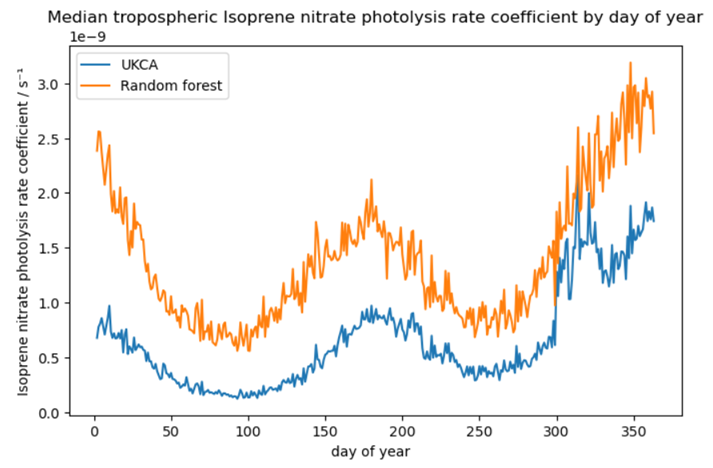
\includegraphics[width=\linewidth]{images/ISON trop med time.png}
    \caption{\textit{Median tropospheric \JISON\ targets and predictions over a year of global, tropospheric test data.}}
    \label{ISON days med}
\end{figure}

% Low altitude problem.
For some reactions, the model performed better in the stratosphere than in the troposphere. The affected reactions were \JOCS, \JISON, \JHHO, \JOOP, \JNNO, \JNO\ and \JmeCHOCHHHH, whose vertical profiles are displayed in appendix \ref{trop problems}. All of these reactions occurred mostly in the stratosphere and had particularly sharp increases in J-value by altitude. The random forest typically made small absolute errors in their predictions, but the errors were significant in the troposphere, where the target values were zero, or close to zero, but the random forest predicted a small positive value, leading to a average over-prediction of these J-values in the troposphere, as illustrated in Figure \ref{ISON days med}.

% Masking method.
Vertical model levels were chosen as a criteria for applying a mask because their values were easy and efficient to check online within the photolysis routines in UKCA. Alternatively, the value of altitude, pressure, downward shortwave flux, SZA or predicted J-value could be used to determine whether or not to apply a mask. The method applied was a hard cut-off, with all values below the masking threshold set to zero and all those above it left unaltered. 

\subection{Final Model Design}

\begin{figure}[htpb]
    \centering 

    % HCHOr corr plot overall (V good).
    \begin{subfigure}{\linewidth}
    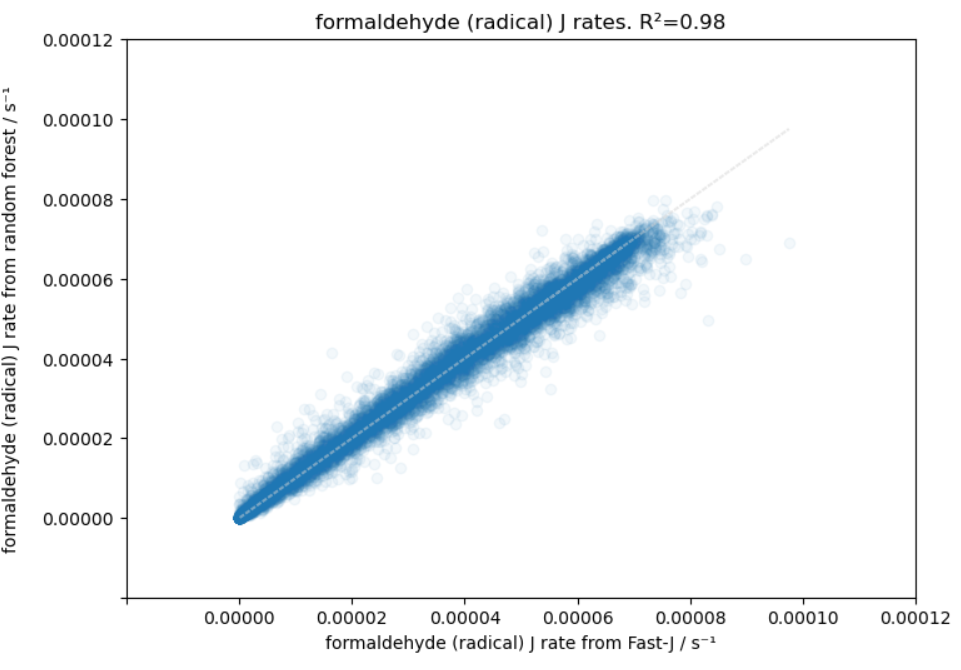
\includegraphics[width=\linewidth]{images/HCHOr.png}
    \caption{\textit{\JHCHOr}}
    \label{HCHOr corr}
    \end{subfigure}

    % Propanal corr plot overall (V good).
    \begin{subfigure}{\linewidth}
    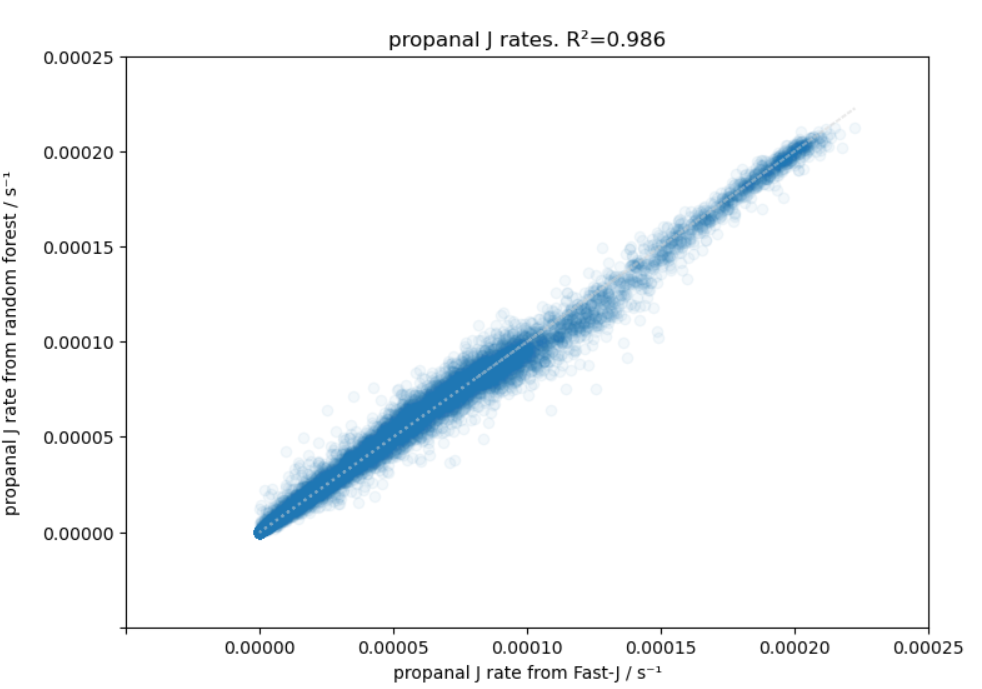
\includegraphics[width=\linewidth]{images/propanal.png}
    \caption{\textit{\Jpropanal}}
    \label{propanal corr}
    \end{subfigure}

    \caption{\textit{Correlation plots of global predictions to targets over a year of test data with a 1:1 reference line.}}
    \label{corr V good}
\end{figure}

% Performance summary.
The random forest performed well, overall, and was capable of emulating both Fast-JX and the 2D lookup table photolysis scheme. Figure \ref{corr V good} shows examples of some of the best-predicted J-values, \JHCHOr\ and \Jpropanal. Most other J-values displayed similarly satisfactory correlations. 
25 out of 26 (96\%) of the emulated reactions achieved \RR\ scores above 0.9. 23 (92\%) of the reactions were emulated with overall global \RR\ scores above 0.95. 13 (50\%) of the reactions were emulated with overall global \RR\ scores above 0.99.

The overall \RR\ score of all predictions to targets from a global, year-long test dataset was 0.97 and the MSE was $3.85 \times 10^{-7}$. The random forest emulated most J-values with \RR\ scores above 0.9, with a few exceptions including 0.79 for \JHHO.

% Best design.
A random forest of few, deep trees was identified as the most effective design for emulating UKCA J-values. The final design chosen included 20 trees of approximately 200,000 nodes each, trained on a one-year dataset of 500,000 uniform randomly sampled data points per day and further randomly sampled at 10\% to 20\% per tree.  
% Sampling.
A large training dataset was shown to be desirable; model performance improved with increasing dataset size up to at least 182 million samples over a year and the global grid.  

% Error.
The random forest performed well for most input feature sets, although it was generally biased to overprediction of small J-values, particularly at low altitudes and in twilight, and biased to underprediction in specific regions. The random forest struggled to predict \JHHO, due to its very small J-values and high altitude of photolysis. 

% Fixes.
Specific J-values were masked to zero at low altitudes to mitigate the overprediction of small J-values at low altitudes. Alternative methods for improving error were identified, including standardising targets and using an ensemble such as a cascaded model or separate models for upper and lower portions of the atmosphere.

\begin{figure}[htpb]
    \centering 

    \begin{subfigure}{\linewidth}
    \centering
    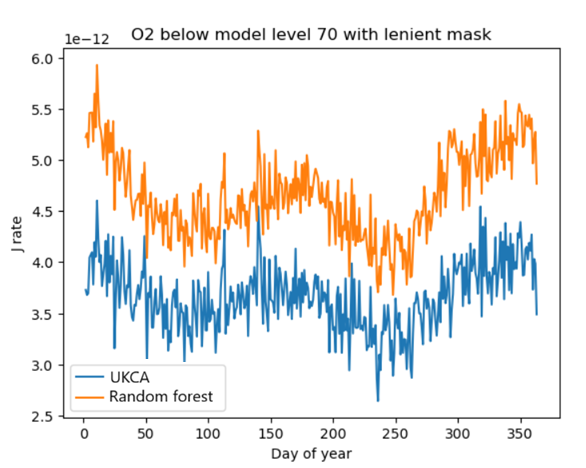
\includegraphics{images/O2 masked preds lenient.png}
    \caption{\textit{\JOOP\ masked too low.}}
    \label{mask too low}
    \end{subfigure}

    \begin{subfigure}{\linewidth}
    \centering
    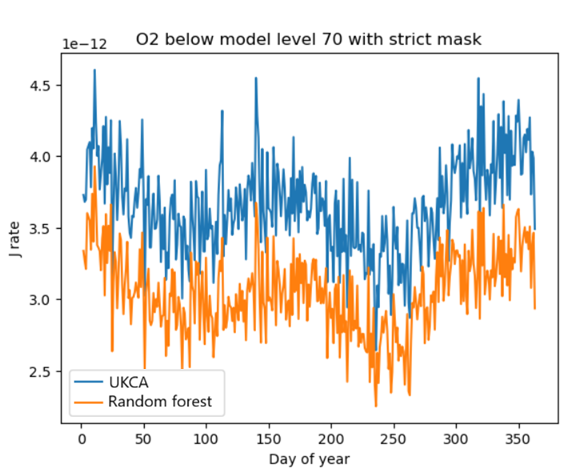
\includegraphics{images/O2 masked preds strict.png}
    \caption{\textit{\JOOP\ masked too high.}}
    \label{mask too high}
    \end{subfigure}

    \caption{\textit{Global daily mean \JOOP\ predictions and targets below model level 70 with too low and too high mask thresholds.}}
    \label{masks high low}
\end{figure}

\begin{table}[htbp]
\centering
\caption{\textit{Model level thresholds for masking J-values to zero. J-values were masked to zero beneath the threshold model level.}}
\begin{tabular}{|lc|}
\hline
Reagent & Level \\
\hline
N$_2$O     & 49 \\
O$_2$      & 50 \\
ISON       & 50 \\
NO         & 52 \\
OCS        & 55 \\
CH$_3$CHO  & 57 \\
H$_2$O     & 61 \\
\hline
\end{tabular}
\label{mask lvls}
\end{table}

% Choosing mask lvls.
Iterative tests were performed in which the maximum level of masking was increased from model levels 50 to 74 and the overall predictive skill and the bias of the mean for each problem J-value were tested. Too low a mask led to the global mean J-values being overpredicted while too high a mask led to mean underprediction; an example of this is shown in Figure \ref{masks high low}. Approaches to choosing the optimal threshold considered the level at which the absolute error reached one order of magnitude, the level at which the mean of the error visually approached zero on a logarithmic scale, the masked level at which the iterative tests produced the best predictions below model level 75, and the best predictions below each masked model level plus five levels above. As displayed in Table \ref{mask lvls}, these tests concluded with model levels 49 to 61 being chosen as the optimal maximum masked levels, depending on each problem reaction, corresponding to points up to the mid-stratosphere. The worst affected J-values required the highest altitude masks, with \JHHO\ being assigned the highest altitude mask and \JNNO\ the lowest. Two approaches to masking were tested: masking predictions to zero and masking training targets to zero. Both approaches produced similar results, demonstrating that very small J-values in the tropospheric training data contributed to the error.

% Decision.
To ensure sufficient time to integrate the model into UKCA and the UM, for a proof of concept, the original random forest was retained, with the option of masking predictions. 

\subsection{The New Photolysis Scheme in UKCA}

% New module.
A proof of concept integration of the random forest into the UM was completed and run. To do this, a new photolysis scheme was added to UKCA, alongside the existing schemes. This new scheme contained a control module and a calculation module. The control module gathered and preprocessed the input data, passed them to the calculation module, and post-processed the output data and returned them to UKCA. On the first photolysis timestep, the calculation module read the random forest's structure from a NetCDF file and reconstructed the model. It then traversed the random forest for every input sample at every photolysis timestep.

% Outputs.
During development and testing, the random forest had been trained to predict the J-values of the reactions of each photolytic species. In UKCA, however, a number of `base' J-values are calculated and mapped to the J-values of each photolysis reaction by multiplying by a constant quantum yield factor, stored in an array in the chemistry master code. Some of the base J-values are reused for multiple reactions of the same functional group. It was necessary to adhere to this process in the new photolysis scheme because the number and order of photolysis reactions performed by UKCA could vary between runs, but the number and order of the random forest's output features were fixed after training. The random forest was altered to output only these required base J-values, which were then mapped to the J-values requested by UKCA. There are a total of 60 base J-values in UKCA but only half of them are used in runs with StratTrop chemistry. The other half would need to be added to the random forest if it were to be applied to CRI-Strat2 chemistry. These base J-values were not included in the outputs of the random forest because they did not correspond to reactions in the UKCA code and were therefore not output in STASH for inclusion in the training dataset. One of the missing base J-values, \JNO, which was not present in the StratTrop chemistry scheme, was present in CRI-Strat2 and its reaction had been encoded in the UKCA chemical master data. Its J-values and reaction flux were added to StratTrop so that they could be output in STASH and the J-value used as an additional training target. Adding \JNO\ was considered particularly desirable because of its role in the $NO_x$ cycle, which strongly influences ozone production and radical chemistry. The other missing base J-values were CRI-Strat2 intermediates, not UKCA photolysis reactions. They were not used for analysis of the proof of concept model's performance in the UM. 

\subsection{Translating the Model to Fortran}

% Constructing NetCDF.
The random forest had been constructed using the Sci-kit Python package and saved as a pickle file. This was not directly translatable to UKCA's code and the pickle file could not be read in Fortran. To address this, the ML model was decomposed into its constituent arrays and saved as a NetCDF file. Arrays were extracted from each decision tree in the constructed, trained random forest, of which feature to check at each node, the threshold to split on at each node, the index of the left child of each node, the index of the right child of each node and prediction values. All of the decision trees were binary, were not pruned, and were the same size and shape, allowing a consistent structure of matching, one-dimensional arrays to represent each component of each tree. Finally, these structural arrays of each tree were compiled as objects in NetCDF format and the whole random forest was saved as a NetCDF file. 

% Reconstructing forest from NetCDF.
Next, an algorithm was written to recreate and traverse each decision tree in the random forest using the data in the NetCDF file's arrays. Sci-kit is open-source software, so its own decision tree traversal code was used as a basis, to ensure consistency \cite{scikit-learn_scikit-learn-180sklearntree_treepyx_2025} \cite{scikit-learn_understanding_2025}. 

% Testing NetCDF.
To ensure correct conversion of the random forest to NetCDF format, the saved NetCDF file was loaded with Python and the random forest was reconstructed using its data, and recreated with Sci-kit. The original random forest was also loaded into Python from the pickle file and the two versions of the random forest were applied to some test data. Both versions output the same predictions, validating the conversion of pickle to NetCDF format.


\section{Results and Analysis}

\subsection{Timings}

\begin{sidewaysfigure}
    \centering 
    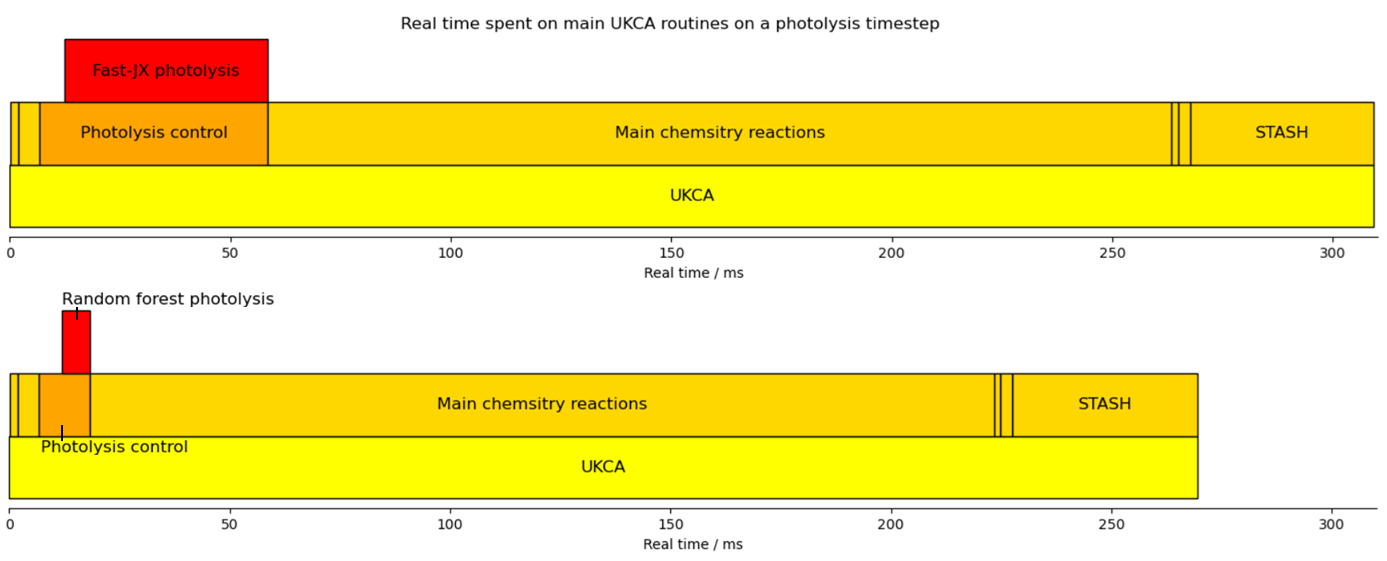
\includegraphics[width=\textheight]{images/Flame FJ ML.png}
    \caption{\textit{UKCA run-time per simulated timestep with StratTrop, using Fast-JX photolysis (top) and random forest photolysis (bottom), to scale.}}
    \label{timings flame}
\end{sidewaysfigure}

\begin{sidewaysfigure}
    \centering 
    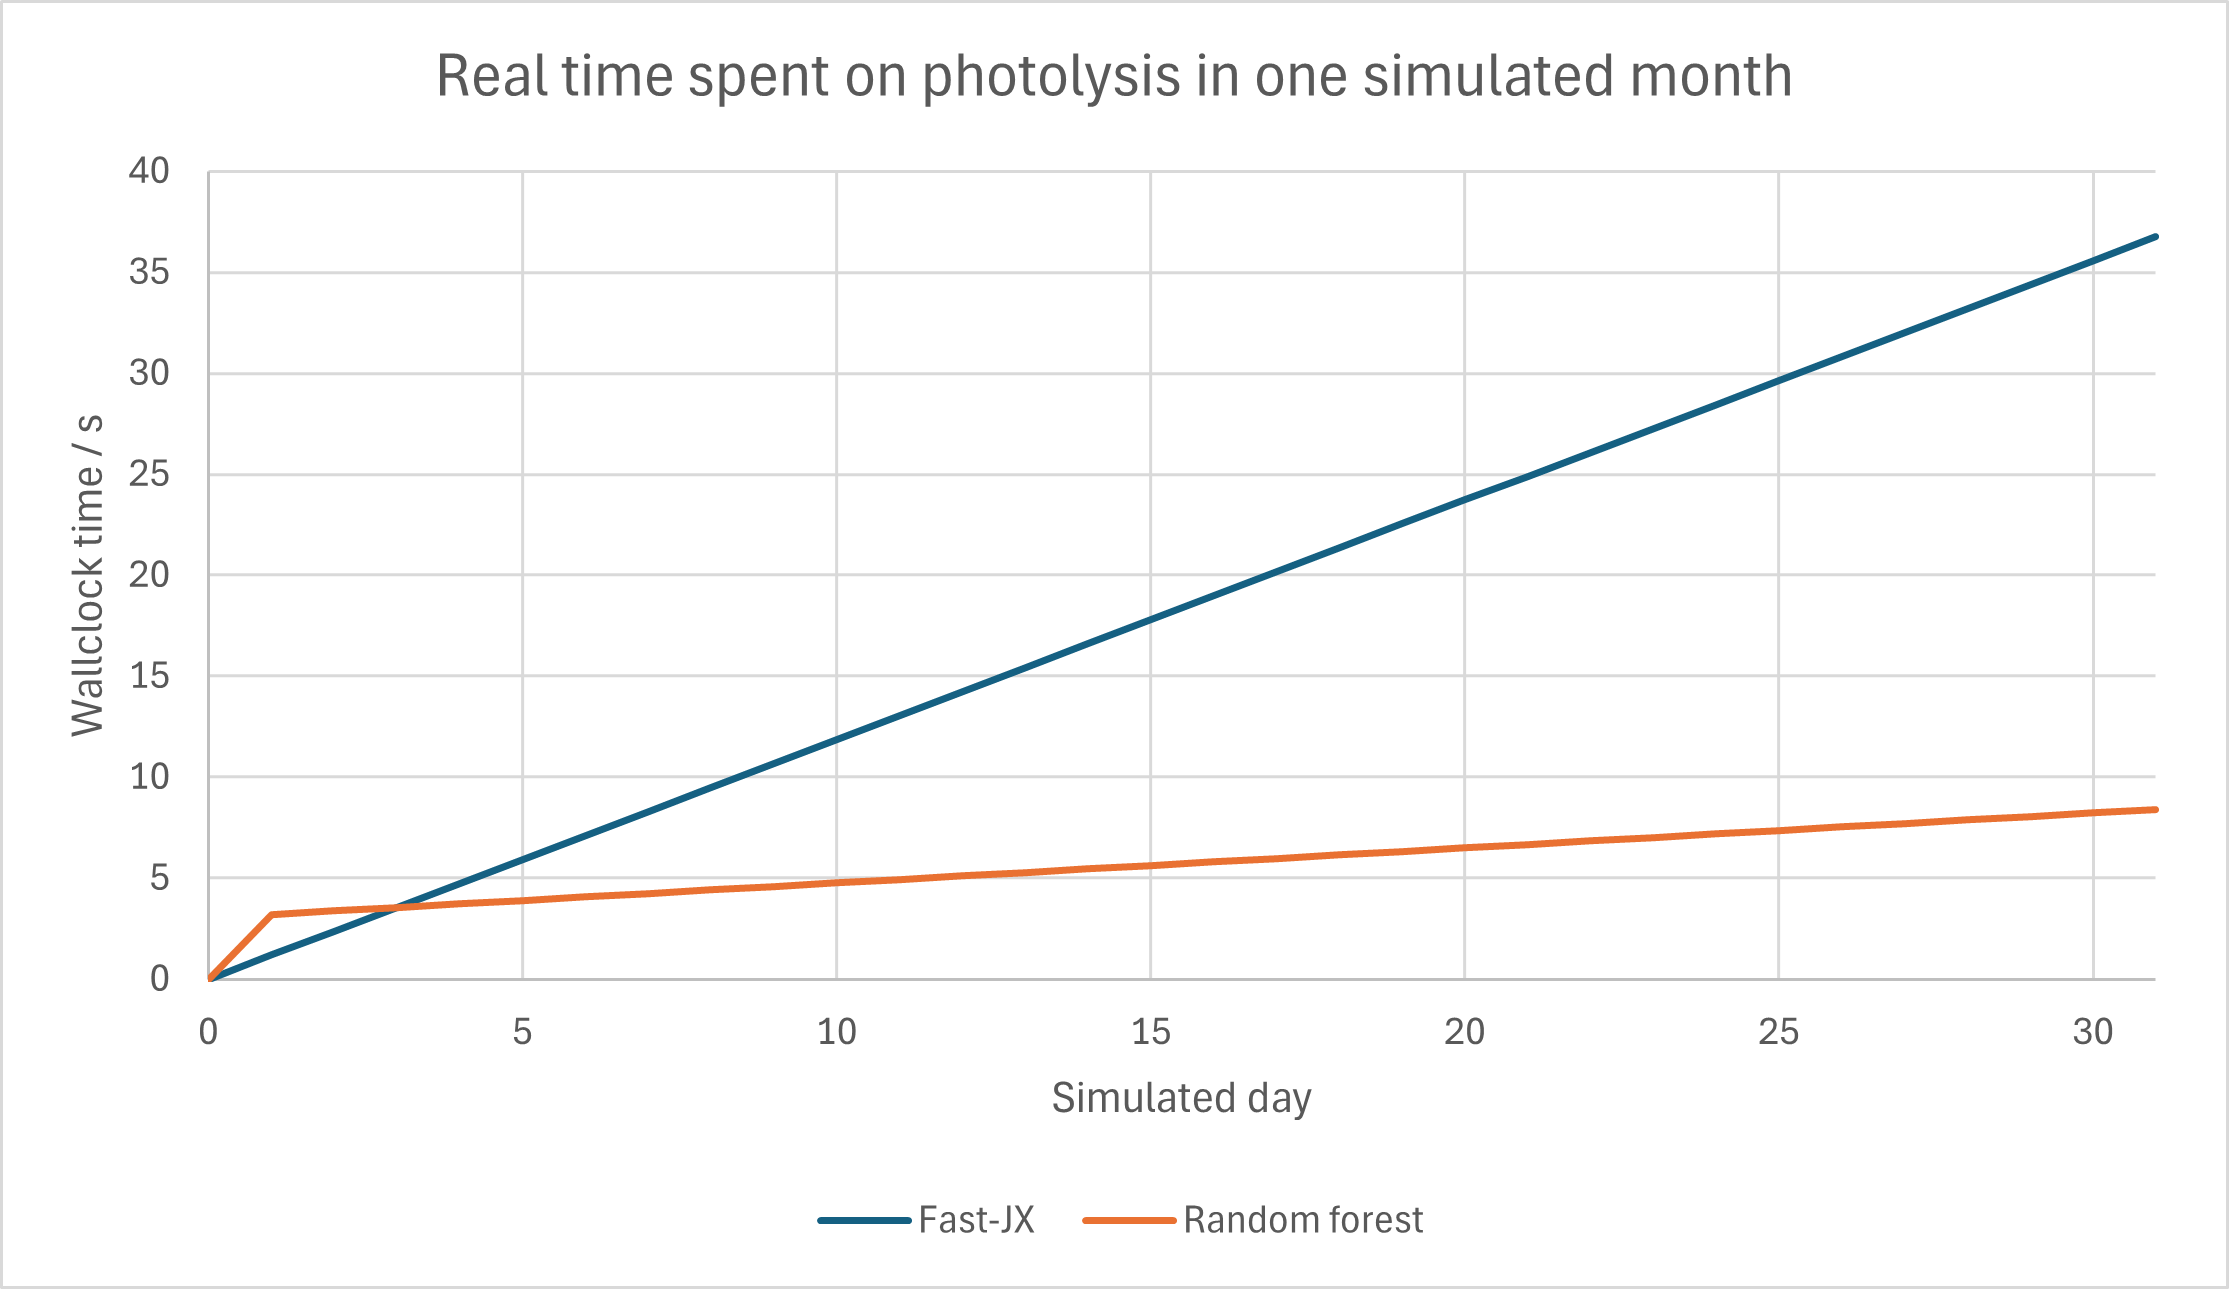
\includegraphics{images/1-month timings.png}
    \caption{\textit{Photolysis run-time per simulated month for Fast-JX and random forest photolysis.}}
    \label{timings plot}
\end{sidewaysfigure}

% Plots.
Figure \ref{timings flame} presents UKCA timings, running StratTrop, for a photolysis timestep using Fast-JX and a photolysis timestep using the random forest implementation. The graphs are to scale and represent all of the UKCA processes in the UM timestep, with routines simplified for ease of presentation and interpretation. The portion labelled `photolysis control' represents processes in the main call to photolysis from the UM to UKCA, which handle data and photolysis requirements and conditions independently of the photolysis scheme. The stratospheric lookup table scheme is included in 'photolysis control' for the Fast-JX version, as it is so fast to run that its timings are negligible. The portion labelled `Fast-JX photolysis' encompasses all of Fast-JX, which has an actual call stack depth of up to 10 routines, including a controller, the SZA calculation, radiation and data handling, as well as the photolysis rate calculation. The portion labelled `random forest photolysis' includes two subroutines: the controller code, which processes data, and the calculation code, which traverses the decision trees. Figure \ref{timings plot} exhibits UKCA's real time spent on photolysis in a simulated month.
 
% Initialisation.
During the first photolysis timestep, the ML photolysis implementation took approximately 60 times longer than the corresponding Fast-JX routines due to initially loading the NetCDF file of large data representing the random forest's structure. Fast-JX has no such initialisation overhead apart from the relatively small burden of allocating and populating persistent arrays. The initial photolysis timestep with Fast-JX took approximately 0.05 seconds, while the initial photolysis timestep with ML photolysis took approximately 3.06 seconds.

% Timings in numbers.
After the first photolysis timestep, the ML photolysis routines ran approximately seven times faster than Fast-JX. Subsequent photolysis timesteps with Fast-JX took approximately 0.05 seconds, and approximately 0.0067 seconds with ML photolysis, on average. Timings for both modules remained stable throughout runs, with a variability range of approximately 4.2 and 1.0 ms for Fast-JX and ML photolysis, respectively. After three simulated days, the cumulative time spent on Fast-JX became longer than the cumulative time spent on ML photolysis. In a simulated month, including the initial photolysis timestep, 8 seconds were spent on ML photolysis, while 36 seconds were spent on Fast-JX. In a simulated year, 66 seconds were spent on ML photolysis, while 433 seconds were spent on Fast-JX. 

\begin{table}[htbp]
\centering
\caption{\textit{Summary of timings and speed-up.}}
\resizebox{\textwidth}{!}{
\begin{tabular}{|lccc|}
\hline
 & Time with Fast-JX / s & Time with ML / s & Run-time \% difference \\
\hline
Initial photolysis timestep     & 0.0549 & 3.0637 & +5477 \\
Subsequent photolysis timesteps & 0.0486 & 0.0067 & -86.21 \\
UKCA photolysis timestep        & 0.3092 & 0.2762 & -10.70 \\
UM photolysis timestep          & 1.1794 & 1.1463 & -2.805 \\
UM simulated hour               & 1.6786 & 1.5524 & -1.971 \\
\hline
\end{tabular}}
\label{timings table}
\end{table}

% Real speedup. 
Table \ref{timings table} lists a summary of timings for both photolysis schemes and percentage speed-ups provided by ML photolysis. `Initial' and `subsequent' `photolysis timesteps' refer to only the photolysis routines. `UKCA photolysis timestep' refers to the same (subsequent) timestep for UKCA including all of the other routines which run on the same timestep as photolysis, shown in figure \ref{timings flame}. `UM photolysis timestep' refers to the same timestep for the UM, containing UKCA, including all of the other routines which run on the same timestep as photolysis. `UM simulated hour' refers to all three hourly UM timesteps including the photolysis timestep. As one in every three UM timesteps are photolysis timesteps in standard configurations, the real speed-up over a model run is a fraction of the speed-up per photolysis timestep; there are 72 timesteps in a simulated day, of which 24 are photolysis timesteps. The main chemistry processes of UKCA are the most time-consuming processes in the UM and photolysis timesteps are by far the most computationally expensive in the UM because they are also the main chemistry timesteps. Both non-photolysis timesteps per simulated hour took approximately 65.4 ms each, while the photolysis timestep, with StratTrop chemistry, took approximately 309 ms with Fast-JX and 276 ms with ML photolysis. Therefore, UKCA photolysis timesteps were 10.7\% faster with the ML approach and the whole of UKCA in total was 7.5\% faster. This is a significant speedup in the context of UKCA performance improvements, such as the 3\% improvement achieved by Esentürk et al. (2018) \cite{esenturk_quasi-newton_2018}. Assuming that UKCA takes up 26.22\% of the UM's run-time, as reported in \cite{dichev_report_2021}, the UM runs approximately 1.97\% faster with ML photolysis than with Fast-JX.

\subsection{Online Predictive Performance}

% Comparing online and offline models.
To test that the random forest behaved as expected in UKCA, the output from the new model run online in UKCA was compared to both UKCA target data and equivalent output data from the random forest run offline in Python. It is typical for models developed offline to exhibit reduced performance when coupled into a larger model and run online, due to feedback mechanisms, error propagation and changes in the input data distribution \cite{stensrud_parameterization_2007}. Apart from some expected differences due to considerations such as timestep offset, numerical precision and data copying in the UM, the random forest produced mostly equivalent predictions in both versions. Due to different conditions and test samples, the online model experienced smaller average J-values than seen in the offline test, but the random forest emulated them relatively accurately.

% Table of results R2.
\begin{sidewaystable}[htbp]
\centering
\caption{\textit{Coefficients of determination of predictions to targets for all J-values emulated online in UKCA over different UM run lengths and spatial regions, along with reference values from the same random forest run offline. Some tropospheric values are missing because those J-values were masked to zero. The values for \JHHO\ are affected by the fact that it was also masked to zero throughout much of the stratosphere.}}
\begin{adjustbox}{max width=\textheight}
\begin{tabular}{|lccccc|}
\toprule
J-values & Offline global mean & 30-year global mean & 1-year global mean & 1-year polar tropospheric mean & 1-year polar stratospheric mean \\
\midrule
CH$_3$ONO$_2$ & 0.996 & 0.995 & 0.944 & 0.957 & 0.933 \\
HNO$_4$       & 0.996 & 0.996 & 0.943 & 0.954 & 0.910 \\
O$_3$         & 0.996 & 0.996 & 0.943 & 0.601 & 0.899 \\
OCS           & 0.995 & 0.996 & 0.942 &  --   & 0.897 \\
SO$_3$        & 0.995 & 0.996 & 0.941 & 0.751 & 0.915 \\
H$_2$O$_2$    & 0.995 & 0.995 & 0.942 & 0.977 & 0.950 \\
CH$_3$OOH     & 0.995 & 0.995 & 0.940 & 0.979 & 0.952 \\
MACROOH       & 0.995 & 0.995 & 0.940 & 0.979 & 0.952 \\
CH$_3$CHO $\rightarrow$ CH$_4$ & 0.995 & 0.996 & 0.943 & -- & 0.665 \\
ISON          & 0.994 & 0.995 & 0.942 & -- & 0.914 \\
HNO$_3$       & 0.994 & 0.995 & 0.946 & 0.507 & 0.912 \\
N$_2$O        & 0.993 & 0.994 & 0.951 & -- & 0.912 \\
CH$_3$CHO $\rightarrow$ CH$_3$O$_2$ & 0.992 & 0.994 & 0.937 & 0.979 & 0.952 \\
Cl$_2$O$_2$   & 0.989 & 0.993 & 0.937 & 0.981 & 0.956 \\
Propanal      & 0.988 & 0.992 & 0.933 & 0.976 & 0.952 \\
NO            & 0.983 & 0.983 & 0.945 & -- & 0.879 \\
HCHOr         & 0.978 & 0.991 & 0.932 & 0.977 & 0.954 \\
HOCl          & 0.977 & 0.990 & 0.934 & 0.981 & 0.955 \\
HCHOm         & 0.975 & 0.993 & 0.935 & 0.981 & 0.954 \\
MACR          & 0.971 & 0.993 & 0.932 & 0.981 & 0.952 \\
NO$_2$        & 0.963 & 0.992 & 0.930 & 0.981 & 0.945 \\
HOBr          & 0.961 & 0.992 & 0.925 & 0.979 & 0.945 \\
CH$_3$COCHO   & 0.950 & 0.991 & 0.922 & 0.977 & 0.938 \\
O$_2 \rightarrow$ O($^3$P) & 0.937 & 0.970 & 0.945 & -- & 0.909 \\
NO$_3$        & 0.917 & 0.982 & 0.906 & 0.968 & 0.925 \\
H$_2$O        & 0.764 & -0.593 & -0.692 & -- & -79.53 \\
\bottomrule
\end{tabular}
\end{adjustbox}
\label{Table R2}
\end{sidewaystable}

% Table of results MSE.
\begin{sidewaystable}[htbp]
\centering
\caption{\textit{MSE, in s$^{-2}$, of predictions to targets for all J-values emulated online in UKCA over different UM run lengths and spatial regions, along with reference values from the same random forest run offline. Some tropospheric values are missing because those J-values were masked to zero. The values for \JHHO\ are affected by the fact that it was also masked to zero throughout much of the stratosphere.}}
\begin{adjustbox}{max width=\textheight}
\sisetup{scientific-notation=true}
\begin{tabular}{|l
S[scientific-notation=true]
S[scientific-notation=true]
S[scientific-notation=true]
S[scientific-notation=true]
S[scientific-notation=true]|}
\toprule
J-values &
{Offline global mean} &
{30-year global mean} &
{1-year global mean} &
{1-year polar tropospheric mean} &
{1-year polar stratospheric mean} \\
\midrule
CH$_3$ONO$_2$        & 2.68e-13 & 1.06e-13 & 2.05e-12 & 3.07e-15 & 1.89e-13 \\
HNO$_4$              & 3.30e-12 & 1.06e-12 & 2.55e-11 & 1.08e-14 & 2.41e-12 \\
O$_3$                & 1.86e-08 & 6.09e-09 & 1.48e-07 & 2.11e-11 & 4.45e-09 \\
OCS                  & 5.97e-13 & 1.79e-13 & 4.27e-12 & {}        & 3.73e-13 \\
SO$_3$               & 8.30e-13 & 2.41e-13 & 5.54e-12 & 1.73e-15 & 9.35e-13 \\
H$_2$O$_2$           & 3.71e-12 & 1.21e-12 & 2.89e-11 & 1.99e-13 & 3.97e-12 \\
CH$_3$OOH            & 1.23e-12 & 3.94e-13 & 9.48e-12 & 1.41e-13 & 1.60e-12 \\
MACROOH              & 3.07e-13 & 9.85e-14 & 2.37e-12 & 3.52e-14 & 3.80e-13 \\
CH$_3$CHO $\rightarrow$ CH$_4$ & 1.26e-14 & 3.77e-15 & 9.24e-14 & {} & 1.62e-15 \\
ISON                 & 7.47e-11 & 2.00e-11 & 4.26e-10 & {} & 1.13e-10 \\
HNO$_3$              & 7.82e-12 & 2.14e-12 & 4.35e-11 & 1.78e-14 & 1.09e-11 \\
N$_2$O               & 2.67e-16 & 6.97e-17 & 1.13e-15 & {} & 3.57e-16 \\
CH$_3$CHO $\rightarrow$ CH$_3$O$_2$ & 1.35e-12 & 3.65e-13 & 8.38e-12 & 2.45e-13 & 2.93e-12 \\
Cl$_2$O$_2$          & 2.76e-08 & 6.21e-09 & 1.45e-07 & 1.10e-08 & 5.66e-08 \\
Propanal             & 4.26e-11 & 9.84e-12 & 1.99e-10 & 1.07e-11 & 1.05e-10 \\
NO                   & 4.51e-15 & 1.42e-15 & 8.16e-15 & {} & 8.48e-17 \\
HCHOr                & 1.20e-11 & 1.62e-12 & 3.94e-11 & 4.88e-12 & 2.99e-11 \\
HOCl                 & 8.24e-10 & 9.85e-11 & 2.99e-09 & 4.21e-10 & 1.97e-09 \\
HCHOm                & 2.30e-11 & 2.15e-12 & 7.56e-11 & 1.26e-11 & 5.53e-11 \\
MACR                 & 1.75e-13 & 1.57e-14 & 5.57e-13 & 9.75e-14 & 4.17e-13 \\
NO$_2$               & 9.00e-07 & 7.59e-08 & 2.65e-06 & 5.18e-07 & 2.14e-06 \\
HOBr                 & 5.72e-08 & 5.17e-09 & 1.68e-07 & 3.31e-08 & 1.29e-07 \\
CH$_3$COCHO          & 9.60e-09 & 1.15e-09 & 2.60e-08 & 5.88e-09 & 2.09e-08 \\
O$_2 \rightarrow$ O($^3$P) & 2.65e-20 & 3.98e-21 & 1.28e-20 & {} & 2.69e-22 \\
NO$_3$               & 9.09e-06 & 6.56e-07 & 1.92e-05 & 6.58e-06 & 1.63e-05 \\
H$_2$O               & 1.83e-13 & 3.69e-13 & 7.11e-13 & {} & 4.64e-18 \\
\bottomrule
\end{tabular}
\end{adjustbox}
\label{Table MSE}
\end{sidewaystable}

% Tables of results.
Tables \ref{Table R2} and \ref{Table MSE} list \RR\ and MSE of every J-value emulated by the proof of concept model online and offline, over different time periods and spatial regions. Most J-values were emulated online with \RR\ scores lower than those of the offline version by approximately 0.05 and resulted in MSE within the same magnitude as in the offline version, in most conditions.

\begin{sidewaysfigure}[htpb]
    \centering 
    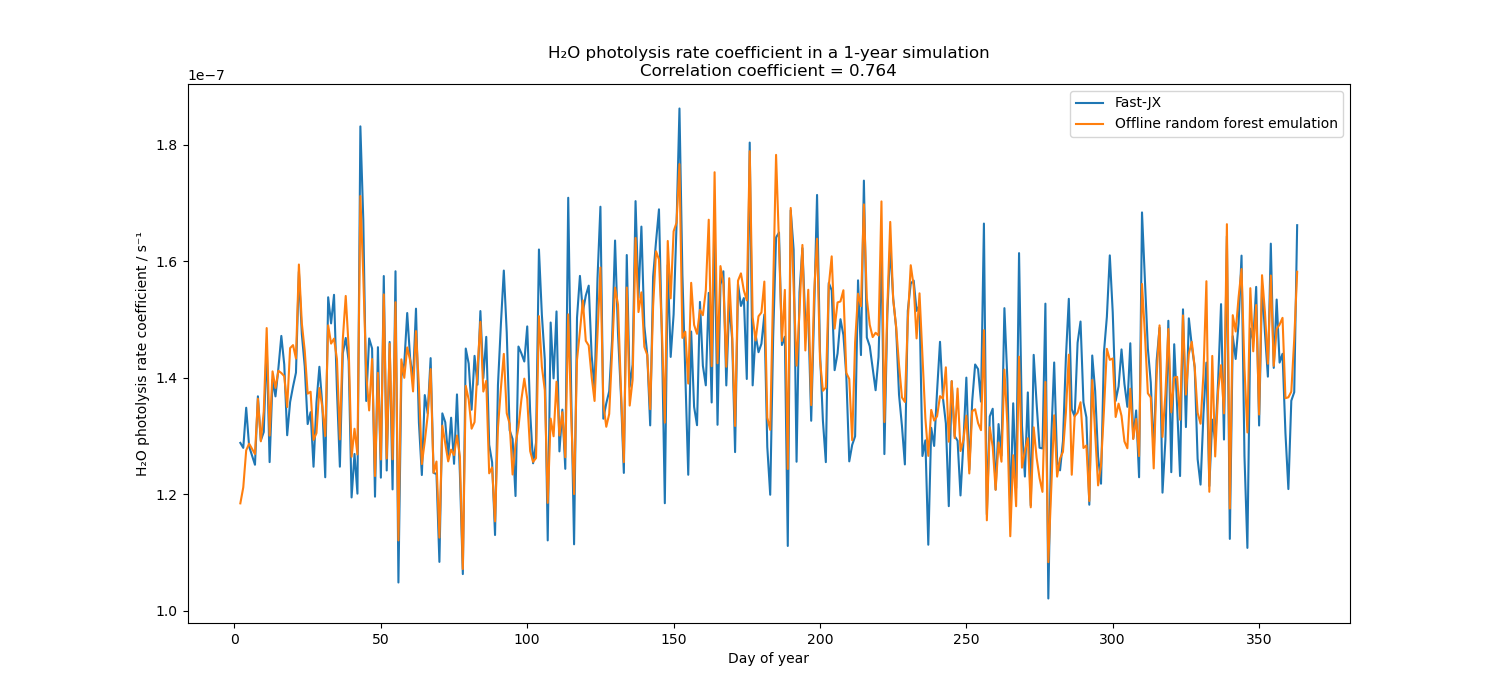
\includegraphics[width=\textheight]{images/H₂O.png}
    \caption{\textit{Global daily mean \JHHO\ targets and predictions from the offline random forest and test dataset, over a year.}}
    \label{Offline H2O day}
\end{sidewaysfigure}

\begin{sidewaysfigure}[htpb]
    \centering 
    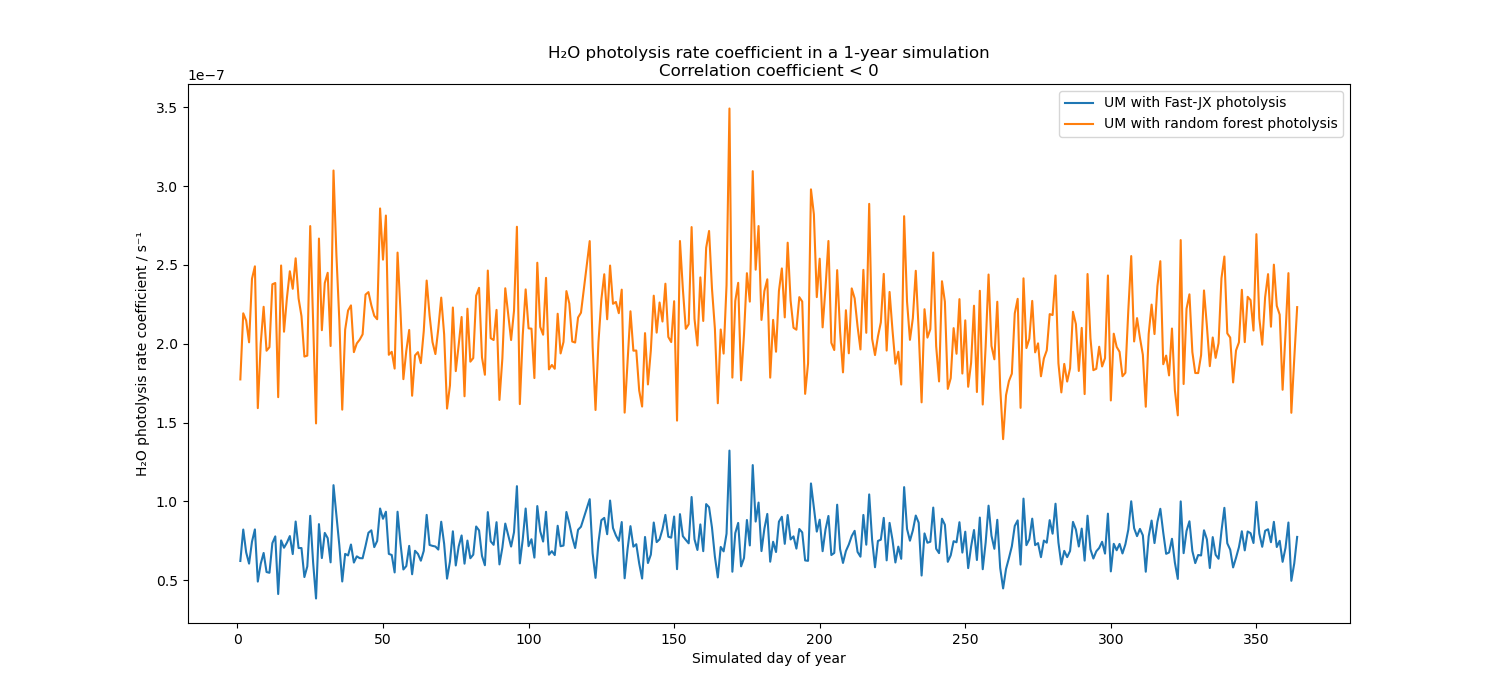
\includegraphics[width=\textheight]{images/H₂O_photolysis rate coefficient.png}
    \caption{\textit{Global daily mean \JHHO\ targets and predictions from an online UKCA simulation of one year with the original and random forest photolysis schemes.}}
    \label{Online H2O day}
\end{sidewaysfigure}

% H2O and other problems.
The main exception to the good online performance was for \JHHO. Figures \ref{Offline H2O day} and \ref{Online H2O day} present \JHHO\ predictions and targets from the offline and online models. The online daily average J-values were persistently biased high by approximately a factor of three, which was not the case in the offline tests. This suggests that the random forest did not capture the full variability in \JHHO\ and that the mask applied offline to \JHHO\ at lower altitudes was not translatable to the different conditions encountered in the online run, especially considering that the mean J-values in the online test sample were lower than the mean of those used for offline training. The online emulated \JHHO\ values fit more closely to the targets in the offline test data, which were considerably higher. This could mean that the distribution of physical inputs seen by the emulator online was outside of its training regime for \JHHO\ evaluation, or the random forest may have been overfit for \JHHO. It could be worth reconsidering the structure of the ML model or its training data for \JHHO. The fact that the \RR\ score of \JHHO\ was lower in the online stratospheric test than in the online global test indicates that the masking to zero at lower altitudes somewhat mitigated the average bias, although the values of \JHHO\ performance are not entirely representative because the mask of zero also extended well into the stratosphere, causing an inevitable discrepancy between emulated outputs and equivalent outputs from the original UKCA photolysis scheme, which were not masked. 
This also applies to \JmeCHOCHHHH, although to a lesser extent, because its mask extended into the stratosphere. This contributed to its relatively low stratospheric \RR\ score of 0.665 when compared to equivalent outputs from the original UKCA photolysis scheme, which were not masked, despite its online stratospheric predictions producing an MSE lower than the offline global MSE.  
\JHNOOO\ displayed a relatively low online tropospheric \RR\ score of 0.507. Similarly to the J-values which were masked to zero at lower altitudes, \JHNOOO\ exhibited a sharp increase in J-value with altitude. It was considered as a candidate for masking, but was not masked due to its lower offline tropospheric error and its smaller potential impact on downstream chemistry. It may be necessary to include \JHNOOO\ in any future plans to resolve low-altitude error in the emulator. 

\subsection{Effect on Downstream Chemistry}

% What things were considered.
To assess the effect of the emulated J-values on downstream science diagnostics in the UM, the mass mixing ratios of chlorine, hydroxyl, water, nitrous oxide, nitric oxide, peroxyacetyl nitrate and ozone were output from the UM, as well as ozone column, O$_x$ production and shortwave heating rates. These diagnostic parameters encompassed the effects of photolysis on radiation, radicals, reservoirs, production and loss in the UM. 

% Cl results.
\begin{sidewaysfigure}[htpb]
    \centering 
    \includegraphics[width=\textheight]{images/Cl_mass mixing ratio.png}
    \caption{\textit{Global daily mean chlorine radical mass mixing ratio from one-year simulations by UKCA with the original and the random forest photolysis schemes.}}
    \label{Cl MMR}
\end{sidewaysfigure}

% Why Cl is useful.
The chlorine radical is representative of halogen radical chemistry, which is sensitive to changes in UV and ozone column \cite{finlayson-pitts_chemistry_2000}. Key reactions include
$Cl_2 + h\nu \rightarrow 2Cl$ and
$ClO + h\nu \rightarrow Cl + O(^3P)$.
% Cl results.
Figure \ref{Cl MMR} displays mean Cl mass mixing ratios over a one-year simulation. UKCA with emulated photolysis produced Cl mass mixing ratios which closely fit those produced by UKCA with the original photolysis scheme, with a slight mean overestimation occurring towards the end of the simulated year. 

% OH results.
\begin{sidewaysfigure}[htpb]
    \centering 
    \includegraphics[width=\textheight]{images/OH_mass mixing ratio.png}
    \caption{\textit{Global daily mean hydroxyl radical mass mixing ratio from one-year simulations by UKCA with the original and the random forest photolysis schemes.}}
    \label{OH MMR}
\end{sidewaysfigure}

% Why OH is useful.
The hydroxyl radical is a primary oxidant in the troposphere and is sensitive to changes to photolysis. The concentration of OH is influenced by many photolysis reaction pathways, especially those involving \OD\ and HO$_x$, and it also affects methane lifetime and VOC chemistry \cite{seinfeld_atmospheric_2016}. Key reactions include 
$O_3 + h\nu \rightarrow O(^1D) + O_2$ and 
$O(^1D) + H_2O \rightarrow 2OH$.
% OH results.
Figure \ref{OH MMR} presents mean OH mass mixing ratios over a year. UKCA with emulated photolysis produced a slight mean overestimation of OH at troughs in the target trend occurring in spring and autumn and more significant overestimation of OH at the global mean peaks in the summers of both hemispheres. The trend over time appeared to have been captured but exaggerated on average. Absolute error was low, however, with a maximum daily MAE of approximately $0.75 \times 10^{-10} s^{-1}$. OH was overestimated to a greater degree in the troposphere than in the stratosphere. This could potentially be improved by further analysing and correcting the effect of water photolysis error and masking. 
% Why OH error could be a problem.
Overestimation of OH could be a significant problem in UKCA because OH is an important sink of several species, including methane, carbon monoxide and VOCs. Altering the concentrations of these species has a series of effects on chemistry throughout UKCA.

% Water results.
\begin{sidewaysfigure}[htpb]
    \centering 
    \includegraphics[width=\textheight]{images/gaps H₂O mass mixing ratio.png}
    \caption{\textit{Global monthly mean water mass mixing ratio from 30-year simulations by UKCA with the original and the random forest photolysis schemes. The gap in 2001 is due to some missing data.}}
    \label{H2O MMR}
\end{sidewaysfigure}

% Why water is useful.
Water photolysis was difficult to emulate due to its small J-values. Water mass mixing ratios were output to determine whether water photolysis errors impacted water in the atmosphere. Water affects OH production via 
$O(^1D) + H_2O \rightarrow 2OH$ \cite{jacob_introduction_1999}.
% Water results.
Figure \ref{H2O MMR} exhibits mean water mass mixing ratios over 30-year simulations. Long model runs were used for water analysis due to the uncertainty of the severity of \JHHO\ error online, according to previous tests. UKCA with emulated photolysis produced similar water mass mixing ratios to those in UKCA with the original photolysis scheme, suggesting that the masking out of low-altitude water photolysis did not harm the mean water content of the atmosphere. This was supported by viewing water over different timescales and in portions of the atmosphere.  

% N2O results.
\begin{sidewaysfigure}[htpb]
    \centering 
    \includegraphics[width=\textheight]{images/gaps N₂O mass mixing ratio.png}
    \caption{\textit{Global monthly mean $N_2O$ mass mixing ratio from 30-year simulations by UKCA with the original and the random forest photolysis schemes. There were some missing data.}}
    \label{N2O MMR}
\end{sidewaysfigure}

% Why N2O is useful.
N$_2$O is useful for viewing effects in the upper atmosphere, as it undergoes photolysis mainly in the stratosphere \cite{world_meteorological_organization_scientific_1998}. Relevant reactions include
$N_2O + h\nu \rightarrow N_2 + O(^1D)$ and
$N_2O + O(^1D) \rightarrow 2NO$.
% N2O results.
Figure \ref{N2O MMR} illustrates mean N$_2$O mass mixing ratios over 30-year simulations. The long model runs show the steady increase of this greenhouse gas over time, attributed to intensifying industrialisation of agriculture and the long lifetime of N$_2$O \cite{tian_global_2024}. Apart from some missing data from both sets, due to technical issues relating to communication with the storage server, UKCA with emulated photolysis reproduced the same overall trend as the original version of UKCA, both annually and over the 30-year test period, although in many months, the global mean was slightly lower than the reference value. 

% NO results.
\begin{sidewaysfigure}[htpb]
    \centering 
    \includegraphics[width=\textheight]{images/NO_mass mixing ratio.png}
    \caption{\textit{Global daily mean NO mass mixing ratio from one-year simulations by UKCA with the original and the random forest photolysis schemes.}}
    \label{NO MMR}
\end{sidewaysfigure}

% Why NO is useful.
NO is a product of NO$_x$ photolysis and affects ozone production \cite{seinfeld_atmospheric_2016}. Some key reactions are
$NO + O_3 \rightarrow NO_2 + O_2$ and
$NO_2 + h\nu \rightarrow NO + O(^3P)$. 
% NO results.
Figure \ref{NO MMR} details daily mean NO mass mixing ratios over a year. UKCA with emulated photolysis contained slightly too much NO on average, globally, throughout the run, although the annual pattern was well represented and the absolute error was low. The excess of NO was more significant in the troposphere than in the stratosphere, indicating that the previously identified tropospheric errors had not been completely mitigated.

% PAN results.
\begin{sidewaysfigure}[htpb]
    \centering 
    \includegraphics[width=\textheight]{images/gaps Peroxyacetyl nitrate mass mixing ratio.png}
    \caption{\textit{Monthly mean global PAN mass mixing ratio from UKCA with the original and random forest photolysis schemes, over a 30-year simulation. There were some missing data for the year 2001.}}
    \label{PAN 30 yr}
\end{sidewaysfigure}

% Why PAN is useful.
Peroxyacetyl nitrate (PAN) is a reservoir for NO$_x$ in the troposphere, affecting ozone and OH in the atmosphere \cite{fischer_atmospheric_2014}. Compared to the other species considered, PAN is more sensitive to temperature, one of the input features for the random forest. An important reaction is
$CH_3COO_2 + NO_2 \ce{<=>} PAN$. PAN is also photolabile but its photolysis reaction is minor and is not yet predicted by the current proof of concept random forest photolysis scheme.
% PAN results.
Figure \ref{PAN 30 yr} presents 30-year monthly mean PAN mass mixing ratios from UKCA running online in the UM with both photolysis schemes. PAN was recorded over a long timescale due to its relatively long lifetime. The random forest slightly underestimated the amplitude of the peaks and troughs on average, but followed the trend well and remained stable throughout the simulation. 

% SW heat results.
\begin{sidewaysfigure}[htpb]
    \centering 
    \includegraphics[width=\textheight]{images/Shortwave heating rates_.png}
    \caption{\textit{Global daily mean shortwave heating rates from one-year simulations by UKCA with the original and the random forest photolysis schemes.}}
    \label{SW heat}
\end{sidewaysfigure}

% Why SW heating is useful.
Shortwave heating rates are used to measure the radiative impact of photolysis changes and are affected by ozone absorption and UV flux changes \cite{hartmann_global_2016}. 
% SW heat results.
Figure \ref{SW heat} exhibits mean shortwave heating rates over a year. The UM with emulated photolysis produced similar shortwave heating rates to those from the UM with the original photolysis version.

% Why O3 MMR, O3 col and Ox prod are useful.
Ozone is particularly important for both photochemistry and radiation and is sensitive to NO$_x$ and HO$_x$ \cite{jacob_introduction_1999}.
Total column ozone affects UV penetration and feeds back to photolysis rates, making it a useful parameter for checking consistency between radiation and photolysis \cite{world_meteorological_organization_scientific_1998}. O$_x$ production measures net ozone production and is an indicator of biases in chemical production rates \cite{finlayson-pitts_chemistry_2000}. Some relevant reactions are 
$NO_2 + h\nu \rightarrow NO + O(^3P)$ and
$O(^3P) + O_2 \rightarrow O_3$.

% O3 MMR results.
\begin{sidewaysfigure}[htpb]
    \centering 
    \includegraphics[width=\textheight]{images/gaps O₃ mass mixing ratio.png}
    \caption{\textit{Global monthly mean ozone mass mixing ratio from 30-year simulations by UKCA with the original and the random forest photolysis schemes. The gaps are due to some missing data.}}
    \label{O3 MMR}
\end{sidewaysfigure}

% O3 MMR results.
Figure \ref{O3 MMR} shows mean ozone mass mixing ratios over 30 years, containing a few portions of missing data. UKCA with emulated photolysis generated similar trends of ozone over time. It moderately underestimated global mean ozone throughout the simulation, although the error remained consistent. This was due to ozone being overestimated in the stratosphere but not at all in the troposphere, potentially implying that the model could benefit from the masking threshold of one or more of the J-values being increased in altitude, or that a smoother transition may be required from zero to the predicted J-values across the masking threshold.

% Ox results.
\begin{sidewaysfigure}[htpb]
    \centering 
    \includegraphics[width=\textheight]{images/gaps Oₓ production .png}
    \caption{\textit{Global monthly mean $O_x$ production from 30-year simulations by UKCA with the original and the random forest photolysis schemes. Some data were missing from the ML output dataset.}}
    \label{Ox prod online}
\end{sidewaysfigure}

% Ox results.
Figure \ref{Ox prod online} presents mean O$_x$ production over 30-year simulations. UKCA with emulated photolysis displayed the same patterns over time as UKCA with the original photolysis scheme, but underestimated O$_x$ production on average throughout the model run. Masking some J-values to zero at low altitudes had been shown to affect O$_x$ production, as presented in Figure \ref{Ox prod lvl mask}, and the low mean bias suggests that this could be further improved.

% Common error.
O$_x$ production and the mass mixing ratios of OH and HO$_2$ displayed similar tendencies to be overestimated at the lower end of their ranges by UKCA with emulated photolysis, corresponding to several reactions whose smallest J-values were overpredicted, including \JHHO.

% CMIP explanation.
The Coupled Model Intercomparison Project Phase 6 (CMIP6) is an co-ordinated international project in which many climate modelling centres around the world run standardised experiments using their Earth System Models \cite{eyring_overview_2016}. It is useful to compare the effects of new changes to a model with data from CMIP6 models because they provide a benchmark of current scientific knowledge and model uncertainty. 

% CMIP.
\begin{sidewaysfigure}[htpb]
    \centering 
    \includegraphics[width=\textheight]{images/gaps CMIP avgs.png}
    \caption{\textit{Monthly mean global ozone over 30-year simulations from different CMIP6 models along with the emulation.}}
    \label{CMIP O3}
\end{sidewaysfigure}

% CMIP models used.
Figure \ref{CMIP O3} exhibits global monthly mean ozone mole fraction over 30-year simulations from AMIP-nudged UM runs with Fast-JX and the stratospheric photolysis scheme, and with the random forest emulation. Three different CMIP6 models were included, which provided ozone data over the required date range for comparison. They include the USA's National Center of Atmospheric Research (NCAR) Community Earth System Model version 2 \cite{danabasoglu_community_2020}, the Centre National de Recherches Météorologiques (CNRM) Earth System Model version 2 \cite{seferian_development_2016}, from France, and the Beijing Climate Center (BCC) Earth System Model version 1 \cite{wu_beijing_2019}, from China. 

% Spin up.
The initial drop in UKCA ozone is due to a relatively long stratospheric ozone spin-up period, which is expected \cite{weber_global_2022}; this plot includes the start of the UM run, which began at January 1982, but the CMIP6 models shown began their simulations at earlier dates and had already completed their spin-up periods before 1982.

% RF analysis.
Variability between downstream ozone mole fraction from UKCA with and without the random forest emulation was less than the variability between different CMIP6 models. UKCA with the photolysis emulation also produced ozone within the existing range of uncertainty between CMIP6 models. This indicates that the emulation produces acceptable effects on online downstream chemistry. 


\conclusions  %% \conclusions[modified heading if necessary]

This proof of concept study has demonstrated that ML can potentially replace atmospheric chemistry models to reduce their computational demand and run time. 
The specific research aims were:\\

1. Identify an appropriate ML model to emulate UKCA photolysis.\\

Several machine learning models of increasing complexity were developed, using physical input features, and compared to a baseline linear regression model.
Simple linear models were unable to capture the intricacies of atmospheric photolysis.
The performance of the ML model generally improved with model complexity, demonstrating that a deep, nonlinear ML method is necessary for predicting the full range of J-values in UKCA.
Decision trees, random forests and neural networks were determined to be suitable for emulating UKCA photolysis, with random forests chosen for this work. 
A large training dataset of UM outputs was necessary, covering all global conditions and times of day and year, occupying at least 8.3 GB. Large decision trees, containing 100,000 leaf nodes, performed better than smaller trees in both standalone decision tree models and as components of a random forest. Shortwave radiation fluxes, SZA and vertical height were important input features for the emulator.\\

2. Use the chosen method to accurately emulate UKCA photolysis rate coefficients, with a global coefficient of determination of at least 0.9 for each emulated reaction.\\

A random forest emulator of UKCA photolysis was designed and evaluated.
The random forest performed well, overall, and was capable of emulating both Fast-JX and the 2D lookup table photolysis scheme. 
The emulator was integrated into the UM and online model output and the effects on downstream chemistry were analysed.
Despite a small drop in accuracy when coupled online, the emulator generally reproduced J-values satisfactorily within UKCA.
25 out of 26 (96\%) of the emulated reactions achieved this aim in both the offline and online models. The only reaction which was not emulated with the desired predictive performance was \JHHO. The small J-values of water photolysis and certain reactions in lower-altitude portions of the atmosphere were particularly difficult to emulate using the chosen method and would be improved by a targeted ensemble of random forests or possibly a neural network.\\

3. Use the chosen model to speed up the run time of UKCA within the UM, reducing the run time of the photolysis portion of UKCA by at least 20\%.\\

This goal was achieved and the target was surpassed, with the implemented emulator reducing the run time of the photolysis portion of UKCA by 85.7\% on all chemistry timesteps except the first, although the emulation was only faster than the original photolysis scheme after 3 simulated days due to its long initialisation time. Converting the emulator from Python to Fortran via a NetCDF file was successful, allowing machine learning models to be trained in Python and integrated into UKCA for online inference. The proof of concept implementation should not currently be used to fully replace the other photolysis schemes in UKCA because not all of UKCA's base J-values have been added to its output set, but this work has demonstrated that it runs successfully in UKCA, predicts most J-values adequately and can be extended to output all base J-values and replace the other photolysis schemes. 

% Performance summary.
The random forest performed well, overall, and was capable of emulating both Fast-JX and the 2D lookup table photolysis scheme.
25 out of 26 (96\%) of the emulated reactions achieved \RR\ scores above 0.9. 23 (92\%) of the reactions were emulated with overall global \RR\ scores above 0.95. 13 (50\%) of the reactions were emulated with overall global \RR\ scores above 0.99.

% Best design.
A random forest of few, deep trees was identified as the most effective design for emulating UKCA J-values. The final design chosen included 20 trees of approximately 200,000 nodes each, trained on a one-year dataset of 500,000 uniform randomly sampled data points per day and further randomly sampled at 10\% to 20\% per tree.  
% Sampling.
A large training dataset was shown to be desirable; model performance improved with increasing dataset size up to at least 182 million samples over a year and the global grid.  

A large training dataset of UM outputs was necessary, covering all global conditions and times of day and year, occupying at least 8.3 GB. Large decision trees, containing 100,000 leaf nodes, performed better than smaller trees in both standalone decision tree models and as components of a random forest. Shortwave radiation fluxes, SZA and vertical height were important input features for the emulator.

% Error.
The random forest performed well for most input feature sets, although it was generally biased to overprediction of small J-values, particularly at low altitudes and in twilight, and biased to underprediction in specific regions. The random forest struggled to predict \JHHO, due to its very small J-values and high altitude of photolysis. 

% Fixes.
Specific J-values were masked to zero at low altitudes to mitigate the overprediction of small J-values at low altitudes

% Timings.
The ML photolysis implementation is faster than Fast-JX in simulations longer than three days. After initialisation, the ML photolysis routines run approximately seven times faster than Fast-JX. The whole UM runs approximately 1.97\% faster with ML photolysis than with Fast-JX.

% What's the accuracy of the emulator when coupled online in the UM?
Despite a small drop in accuracy when coupled online, the emulator generally reproduced J-values well within UKCA. With the exception of \JHHO, most online emulated outputs exceeded the target \RR\ score of 0.9 and resulted in MSE within the same magnitude as in the offline version, in most conditions and regions of space.

% What's its effect on key chemical fields?
The overprediction of a specific set of J-values at low altitudes was shown to have a greater effect on downstream chemistry than anticipated, particularly on OH concentrations, although ozone column data remained within the range of uncertainty displayed between CMIP6 models.

% Is the trade-off between accuracy and performance acceptable?
The trade-off between accuracy and performance may be acceptable depending on the importance of photolysis-related chemistry in each use of the UM. The current design of the emulator could be used as a faster alternative to Fast-JX for long model runs in which effects of photolysis are not a top priority, but ideally, the emulator should be improved further to address \JHHO\ and low-altitude issues and achieve its potential accuracy. 


%% The following commands are for the statements about the availability of data sets and/or software code corresponding to the manuscript.
%% It is strongly recommended to make use of these sections in case data sets and/or software code have been part of your research the article is based on.


\codedataavailability{
Data samples and scripts to reproduce results can be found at the following locations.\\
Python scripts: \url{https://github.com/Sophie-Turner/Sophies_UKCA_scripts}\\
Zenodo data sample: \url{https://zenodo.org/records/20307039}\\
The code changes implemented in UKCA can also be viewed for reference.\\
UKCA branch: \url{https://github.com/Sophie-Turner/ukca/tree/um13.9_ukca_dev/src/science/photolysis/ml}
}


\appendix
\section{}    %% Appendix A

\subsection{}     %% Appendix A1, A2, etc.


\noappendix       %% use this to mark the end of the appendix section. Otherwise the figures might be numbered incorrectly (e.g. 10 instead of 1).

%% Regarding figures and tables in appendices, the following two options are possible depending on your general handling of figures and tables in the manuscript environment:

%% Option 1: If you sorted all figures and tables into the sections of the text, please also sort the appendix figures and appendix tables into the respective appendix sections.
%% They will be correctly named automatically.

%% Option 2: If you put all figures after the reference list, please insert appendix tables and figures after the normal tables and figures.
%% To rename them correctly to A1, A2, etc., please add the following commands in front of them:

\appendixfigures  %% needs to be added in front of appendix figures

\appendixtables   %% needs to be added in front of appendix tables

%% Please add \clearpage between each table and/or figure. Further guidelines on figures and tables can be found below.



\authorcontribution{TEXT} %% this section is mandatory

\competinginterests{TEXT} %% this section is mandatory even if you declare that no competing interests are present

\disclaimer{TEXT} %% optional section

\begin{acknowledgements}
This work was supported by the UKRI Centre for Doctoral Training in Application of Artificial Intelligence to the study of Environmental Risks (reference EP/S022961/1).
\end{acknowledgements}




%% REFERENCES

%% The reference list is compiled as follows:

\begin{thebibliography}{}

\bibitem[AUTHOR(YEAR)]{LABEL1}
REFERENCE 1

\bibitem[AUTHOR(YEAR)]{LABEL2}
REFERENCE 2

\end{thebibliography}

%% Since the Copernicus LaTeX package includes the BibTeX style file copernicus.bst,
%% authors experienced with BibTeX only have to include the following two lines:
%%
%% \bibliographystyle{copernicus}
%% \bibliography{example.bib}
%%
%% URLs and DOIs can be entered in your BibTeX file as:
%%
%% URL = {http://www.xyz.org/~jones/idx_g.htm}
%% DOI = {10.5194/xyz}


%% LITERATURE CITATIONS
%%
%% command                        & example result
%% \citet{jones90}|               & Jones et al. (1990)
%% \citep{jones90}|               & (Jones et al., 1990)
%% \citep{jones90,jones93}|       & (Jones et al., 1990, 1993)
%% \citep[p.~32]{jones90}|        & (Jones et al., 1990, p.~32)
%% \citep[e.g.,][]{jones90}|      & (e.g., Jones et al., 1990)
%% \citep[e.g.,][p.~32]{jones90}| & (e.g., Jones et al., 1990, p.~32)
%% \citeauthor{jones90}|          & Jones et al.
%% \citeyear{jones90}|            & 1990



%% FIGURES

%% When figures and tables are placed at the end of the MS (article in one-column style), please add \clearpage
%% between bibliography and first table and/or figure as well as between each table and/or figure.

% The figure files should be labelled correctly with Arabic numerals (e.g. fig01.jpg, fig02.png).


%% ONE-COLUMN FIGURES

%%f
%\begin{figure}[t]
%\includegraphics[width=8.3cm]{FILE NAME}
%\caption{TEXT}
%\end{figure}
%
%%% TWO-COLUMN FIGURES
%
%%f
%\begin{figure*}[t]
%\includegraphics[width=12cm]{FILE NAME}
%\caption{TEXT}
%\end{figure*}
%
%
%%% TABLES
%%%
%%% The different columns must be seperated with a & command and should
%%% end with \\ to identify the column brake.
%
%%% ONE-COLUMN TABLE
%
%%t
%\begin{table}[t]
%\caption{TEXT}
%\begin{tabular}{column = lcr}
%\tophline
%
%\middlehline
%
%\bottomhline
%\end{tabular}
%\belowtable{} % Table Footnotes
%\end{table}
%
%%% TWO-COLUMN TABLE
%
%%t
%\begin{table*}[t]
%\caption{TEXT}
%\begin{tabular}{column = lcr}
%\tophline
%
%\middlehline
%
%\bottomhline
%\end{tabular}
%\belowtable{} % Table Footnotes
%\end{table*}
%
%%% LANDSCAPE TABLE
%
%%t
%\begin{sidewaystable*}[t]
%\caption{TEXT}
%\begin{tabular}{column = lcr}
%\tophline
%
%\middlehline
%
%\bottomhline
%\end{tabular}
%\belowtable{} % Table Footnotes
%\end{sidewaystable*}
%
%
%%% MATHEMATICAL EXPRESSIONS
%
%%% All papers typeset by Copernicus Publications follow the math typesetting regulations
%%% given by the IUPAC Green Book (IUPAC: Quantities, Units and Symbols in Physical Chemistry,
%%% 2nd Edn., Blackwell Science, available at: http://old.iupac.org/publications/books/gbook/green_book_2ed.pdf, 1993).
%%%
%%% Physical quantities/variables are typeset in italic font (t for time, T for Temperature)
%%% Indices which are not defined are typeset in italic font (x, y, z, a, b, c)
%%% Items/objects which are defined are typeset in roman font (Car A, Car B)
%%% Descriptions/specifications which are defined by itself are typeset in roman font (abs, rel, ref, tot, net, ice)
%%% Abbreviations from 2 letters are typeset in roman font (RH, LAI)
%%% Vectors are identified in bold italic font using \vec{x}
%%% Matrices are identified in bold roman font
%%% Multiplication signs are typeset using the LaTeX commands \times (for vector products, grids, and exponential notations) or \cdot
%%% The character * should not be applied as mutliplication sign
%
%
%%% EQUATIONS
%
%%% Single-row equation
%
%\begin{equation}
%
%\end{equation}
%
%%% Multiline equation
%
%\begin{align}
%& 3 + 5 = 8\\
%& 3 + 5 = 8\\
%& 3 + 5 = 8
%\end{align}
%
%
%%% MATRICES
%
%\begin{matrix}
%x & y & z\\
%x & y & z\\
%x & y & z\\
%\end{matrix}
%
%
%%% ALGORITHM
%
%\begin{algorithm}
%\caption{...}
%\label{a1}
%\begin{algorithmic}
%...
%\end{algorithmic}
%\end{algorithm}
%
%
%%% CHEMICAL FORMULAS AND REACTIONS
%
%%% For formulas embedded in the text, please use \chem{}
%
%%% The reaction environment creates labels including the letter R, i.e. (R1), (R2), etc.
%
%\begin{reaction}
%%% \rightarrow should be used for normal (one-way) chemical reactions
%%% \rightleftharpoons should be used for equilibria
%%% \leftrightarrow should be used for resonance structures
%\end{reaction}
%
%
%%% PHYSICAL UNITS
%%%
%%% Please use \unit{} and apply the exponential notation (e.g. 20\,\unit{W\,m^{-2}})


\end{document}
